% $Header: /home/vedranm/bitbucket/beamer/solutions/conference-talks/conference-ornate-20min.en.tex,v 90e850259b8b 2007/01/28 20:48:30 tantau $

\documentclass{beamer}


\mode<presentation>
{
  \usetheme{Warsaw}
  %\usetheme{default}
  % or ...

  \setbeamercovered{transparent}
  % or whatever (possibly just delete it)
}


\usepackage[english]{babel}
% or whatever

\usepackage[latin1]{inputenc}
% or whatever

\usepackage{times}
\usepackage[T1]{fontenc}
\usepackage{amsmath}
\usepackage{epstopdf}
% Or whatever. Note that the encoding and the font should match. If T1
% does not look nice, try deleting the line with the fontenc.


\title[Recent results and discussions] % (optional, use only with long paper titles)
{Landauer Experiment \\Recent results and discussions}


%\author[Shreyas Bhaban]{Shreyas Bhaban}% (optional, use only with lots of authors)

\institute[U of M] % (optional, but mostly needed)
{
 Department of Electrical Engineering\\
 University of Minnesota\\
}
% - Use the \inst command only if there are several affiliations.
% - Keep it simple, no one is interested in your street address.

\date{\today}



\AtBeginSubsection[]
{
  \begin{frame}<beamer>{Outline}
    \tableofcontents[currentsection,currentsubsection]
  \end{frame}
}


\begin{document}

\begin{frame}
  \titlepage
\end{frame}

\begin{frame}{Outline}
  \tableofcontents  % You might wish to add the option [pausesections]
\end{frame}

%%-----------------------------------------------------------------------------------------------------------------
\section{Potential well construction}
\begin{frame}{Double well- I4k, 800, right, 10, 5} 
SD = 47.8 nm
\begin{figure}
    \centering
    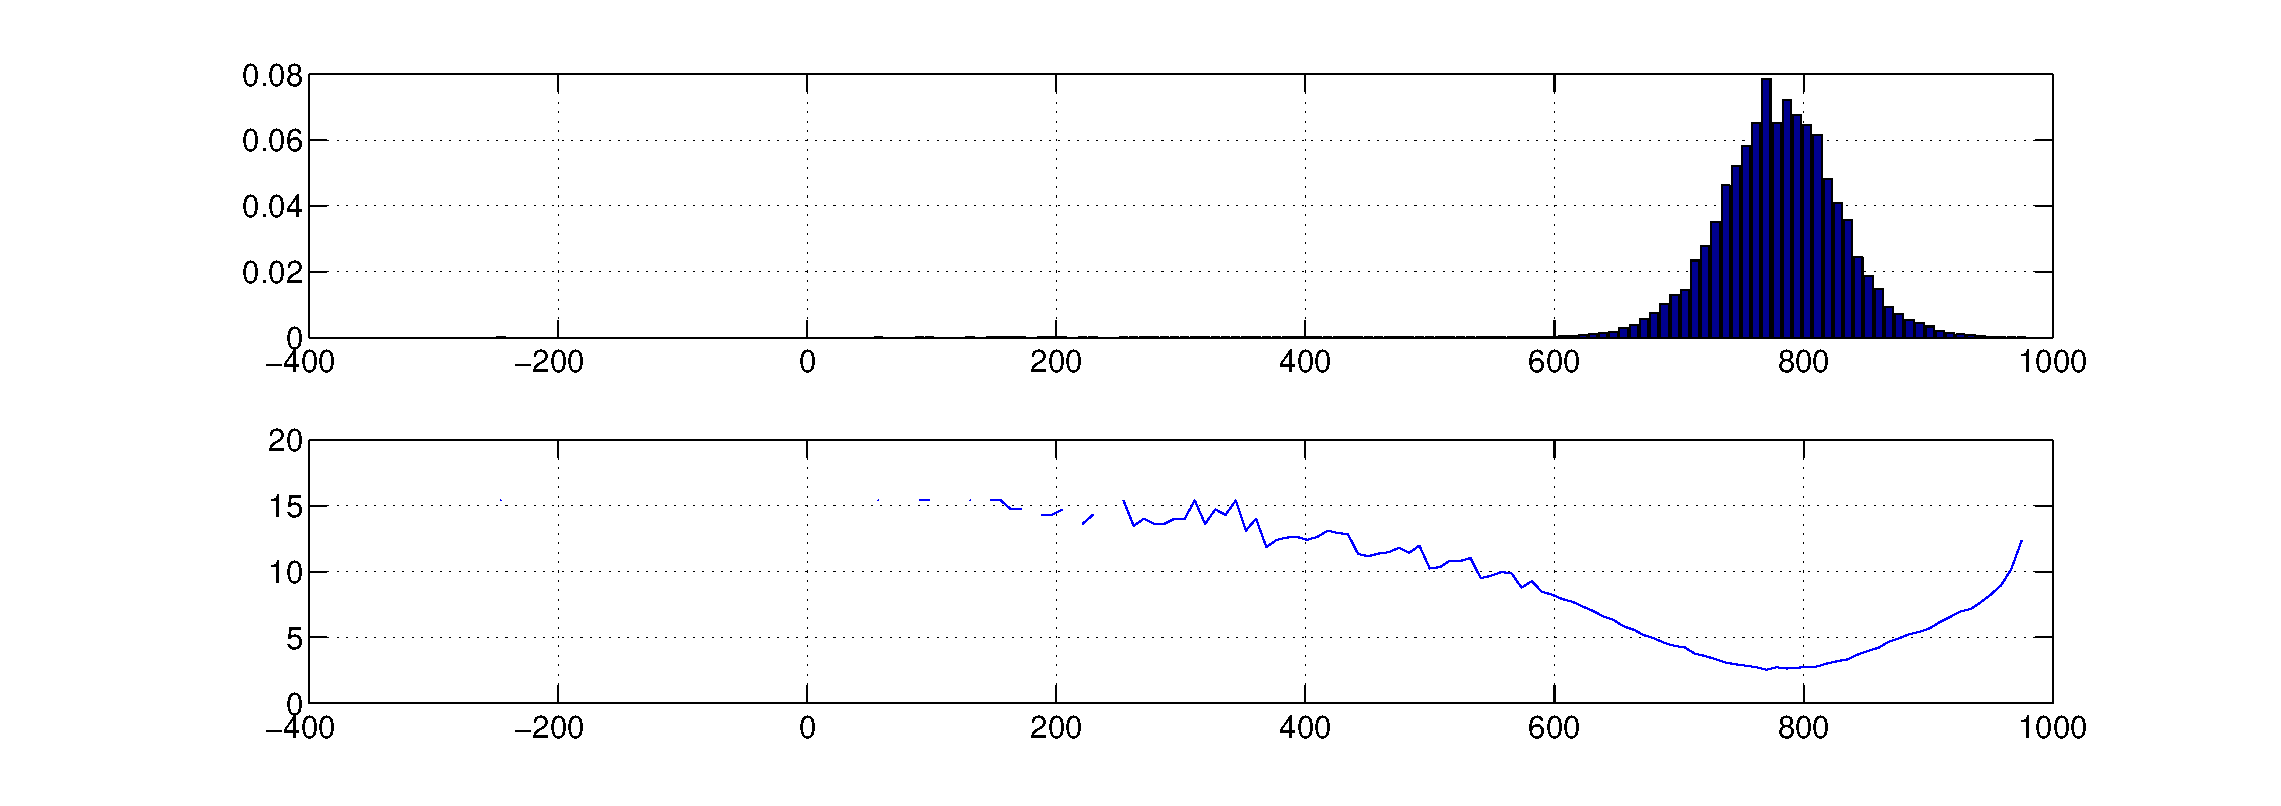
\includegraphics[height=5cm,width=12cm]{right_well_I4k_800.eps}
%    \caption{Applying step fitting to bead trace}
    \label{fig:graph1}
\end{figure}


\end{frame}

%%-----------------------------------------------------------------------
\begin{frame}{Double well- I4k, 800, left, 10, 5} 
SD = 57.8 nm
\begin{figure}
    \centering
    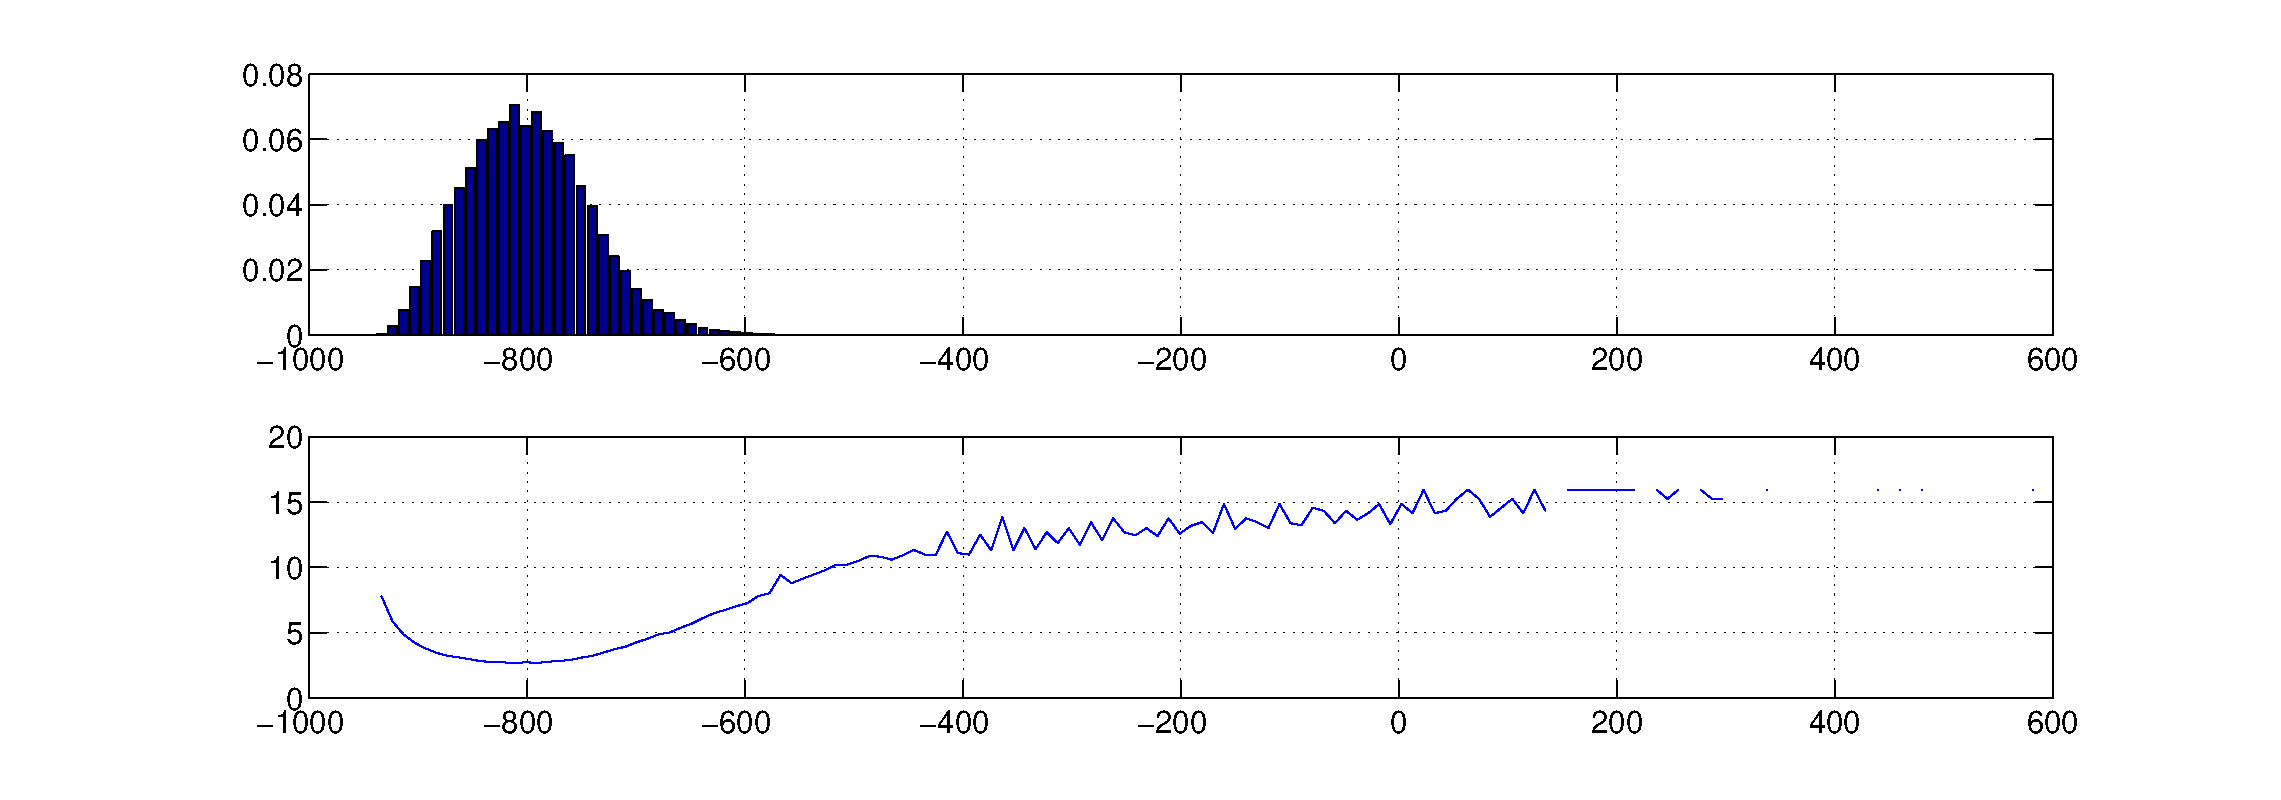
\includegraphics[height=5cm,width=12cm]{left_well_I4k_800.eps}
    \caption{Applying step fitting to bead trace}
    \label{fig:graph2}
\end{figure}


\end{frame}

%%-----------------------------------------------------------------------
\begin{frame}{Double well- I4k, 800, Both, 10, 5} 
R=2.625 $K_BT$, L = 2.675 $K_BT$ 
\begin{figure}
    \centering
    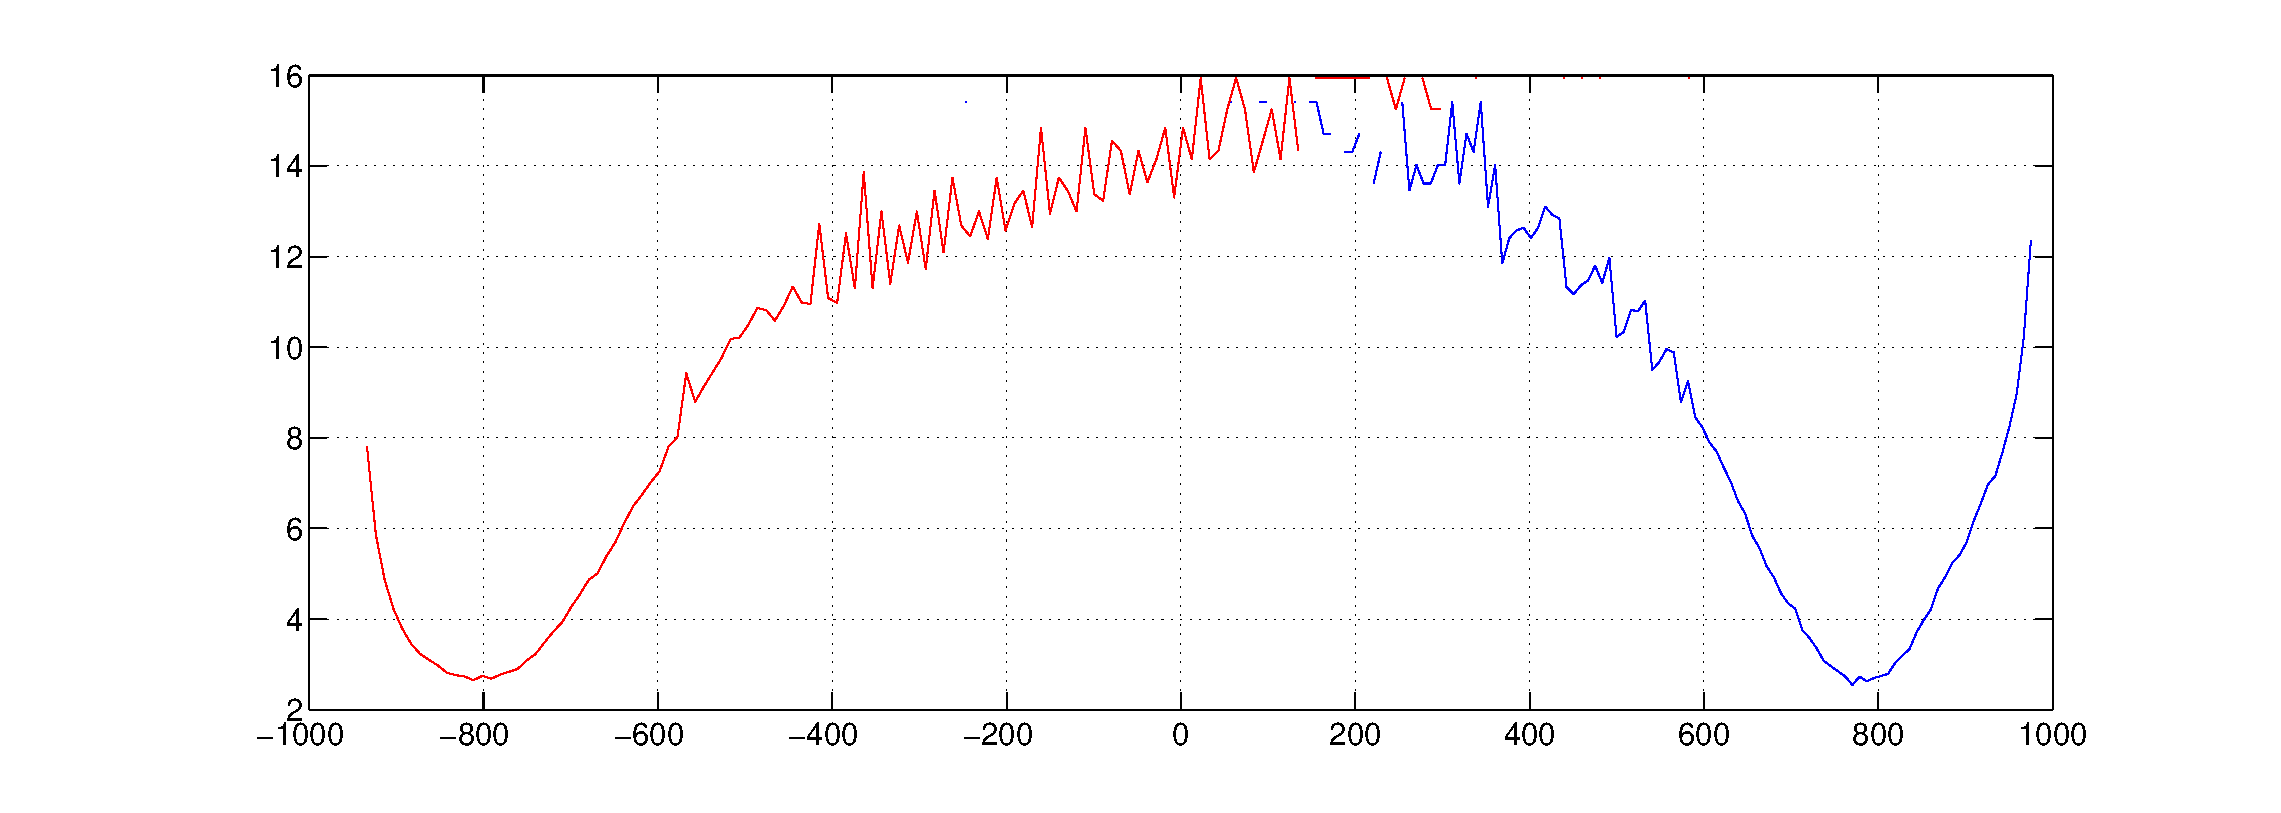
\includegraphics[height=5cm,width=12cm]{both_wells_800_I4k.eps}
    \caption{Applying step fitting to bead trace}
    \label{fig:graph3}
\end{figure}


\end{frame}

%%-----------------------------------------------------------------------
\begin{frame}{Double well- I800, 800, right, 10, 5} 
SD= 367.71 nm, Depth= 3.3 $K_BT$ 
\begin{figure}
    \centering
    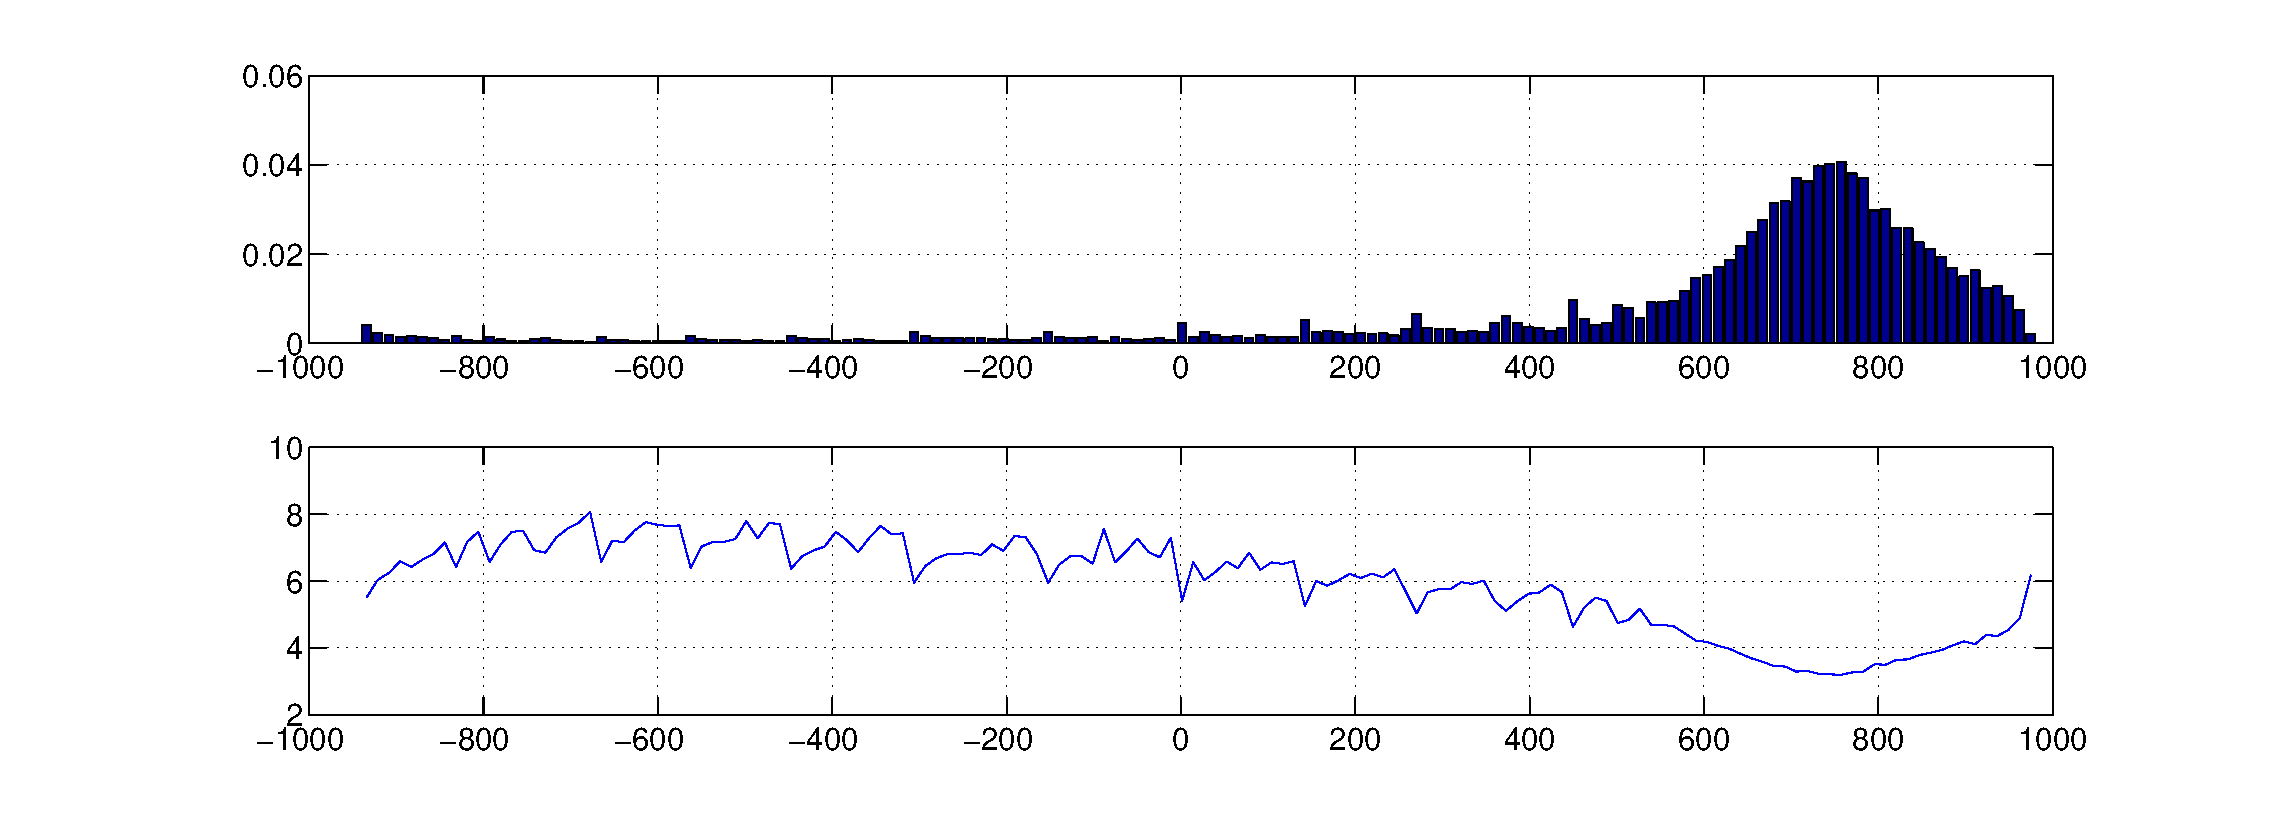
\includegraphics[height=5cm,width=12cm]{right_well_I800_800.eps}
    \caption{Applying step fitting to bead trace}
    \label{fig:graph4}
\end{figure}


\end{frame}



%%-----------------------------------------------------------------------
\begin{frame}{Double well- I4k, 700, both, 10, 5} 
R=2.2 $K_BT$, SD = 36.1 nm, L = 3 $K_BT$, SD = 52.3 nm 
\begin{figure}
    \centering
    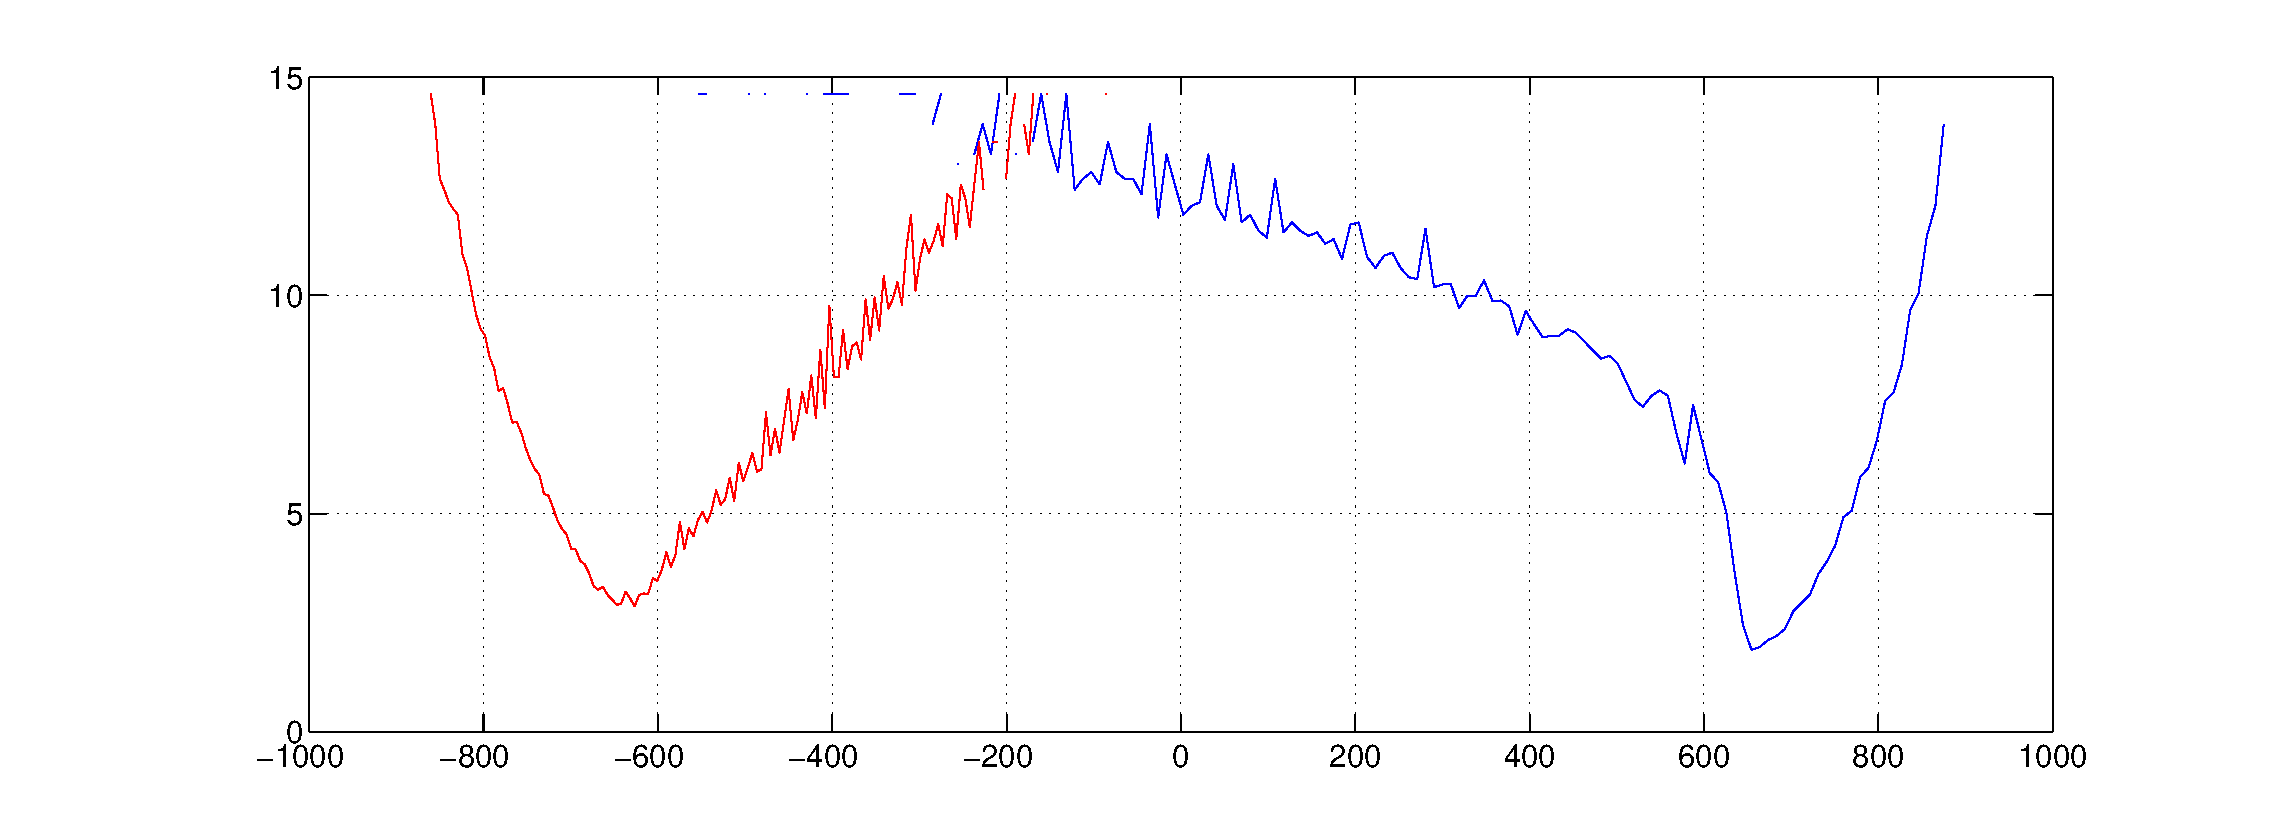
\includegraphics[height=5cm,width=12cm]{both_wells_I4k_700.eps}
%    \caption{Applying step fitting to bead trace}
    \label{fig:graph5}
\end{figure}


\end{frame}

%%-----------------------------------------------------------------------
\begin{frame}{Double well- I1.5k, 700, right, 10, 5} 
SD = 45.9 nm
\begin{figure}
    \centering
    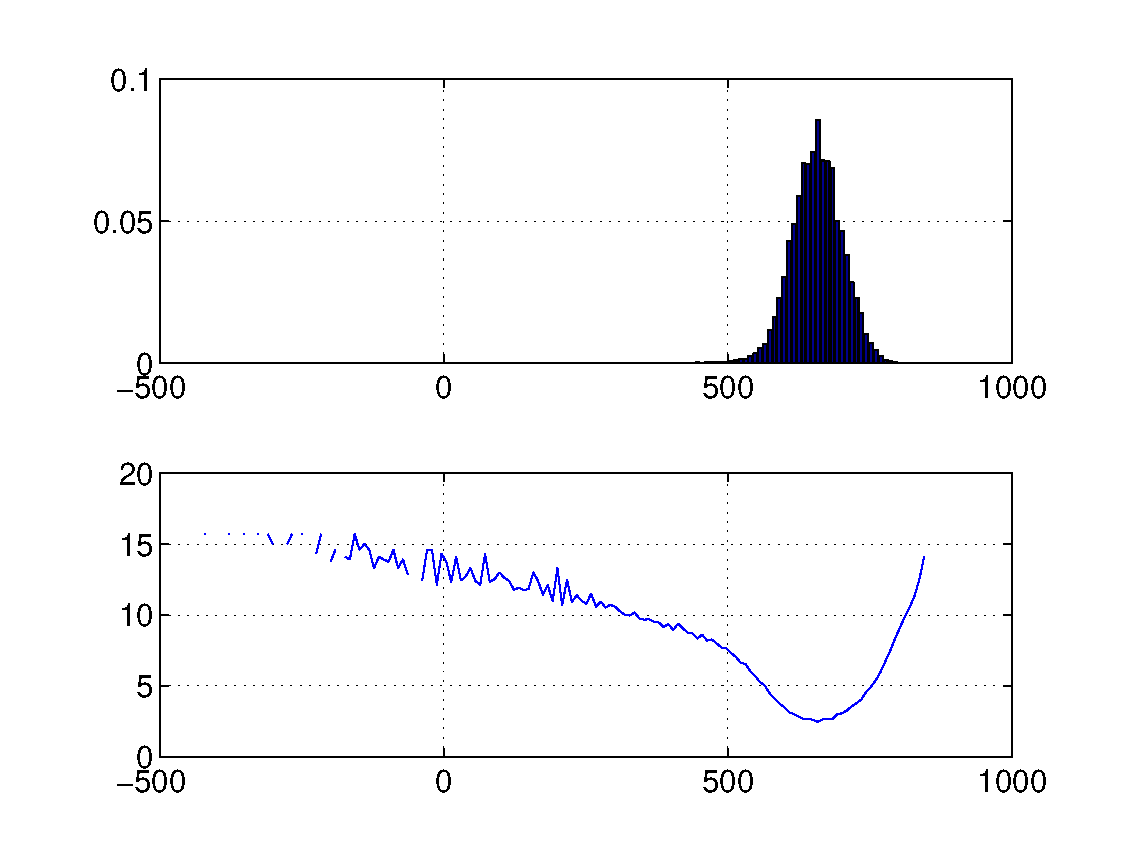
\includegraphics[height=5cm,width=12cm]{right_well_1_5k_700_3.eps}
%    \caption{Applying step fitting to bead trace}
    \label{fig:graph6}
\end{figure}


\end{frame}

%%-----------------------------------------------------------------------
\begin{frame}{Double well- I1.5k, 700, left, 10, 5} 
SD = 53.22 nm 
\begin{figure}
    \centering
    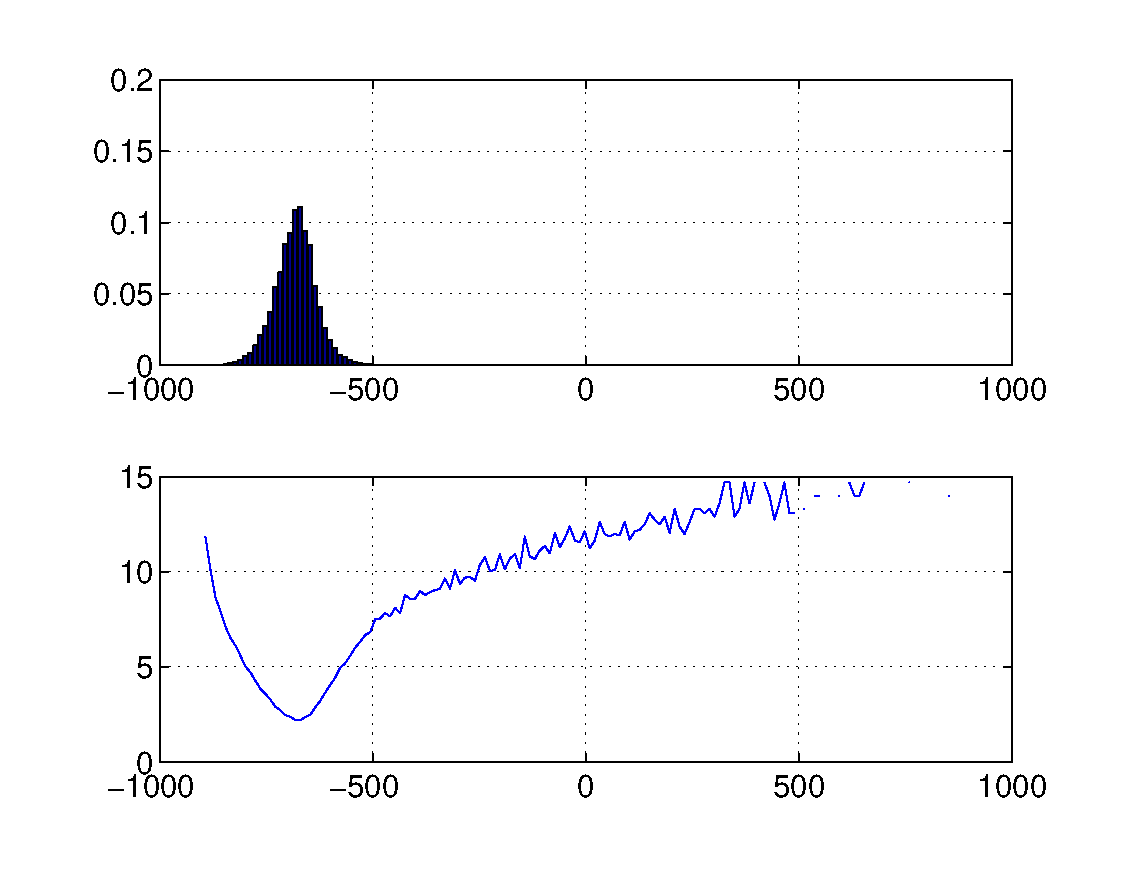
\includegraphics[height=5cm,width=12cm]{left_well_1_5k_700_9.eps}
 %   \caption{Applying step fitting to bead trace}
    \label{fig:graph7}
\end{figure}


\end{frame}

%%-----------------------------------------------------------------------
\begin{frame}{Double well- I1.5k, 700, both, 10, 5} 
R=2.6 $K_BT$, L = 2.2 $K_BT$
\begin{figure}
    \centering
    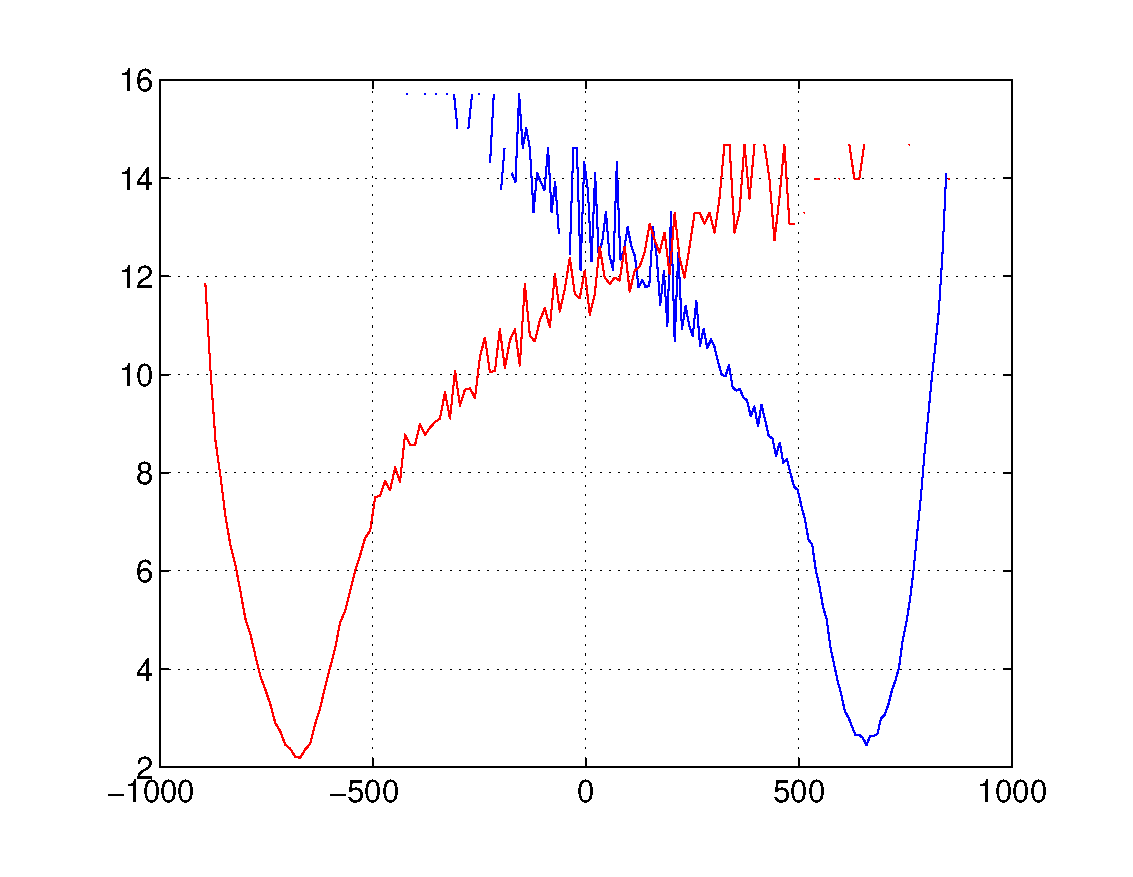
\includegraphics[height=5cm,width=12cm]{both_wells_1_5k_700_3and9.eps}
 %   \caption{Applying step fitting to bead trace}
    \label{fig:graph8}
\end{figure}


\end{frame}
%%--------------------------------------------------------------------------------------------------------
%%-----------------------------------------------------------------------
\begin{frame}{Double well- I1.5k, 700, right, 10, 5} 
SD = 65.6 nm
\begin{figure}
    \centering
    \includegraphics[height=5cm,width=12cm]{right_well_I1_5k_700_4.eps}
    \caption{Applying step fitting to bead trace}
    \label{fig:graph9}
\end{figure}


\end{frame}

%%-----------------------------------------------------------------------
\begin{frame}{Double well- I1.5k, 700, left, 10, 5} 
SD = 53.05 nm 
\begin{figure}
    \centering
    \includegraphics[height=5cm,width=12cm]{left_well_I1_5k_700_3.eps}
%    \caption{Applying step fitting to bead trace}
    \label{fig:graph10}
\end{figure}


\end{frame}

%%-----------------------------------------------------------------------
\begin{frame}{Double well- I1.5k, 700, both, 10, 5} 
R=2.35 $K_BT$, L = 2.3 $K_BT$
\begin{figure}
    \centering
    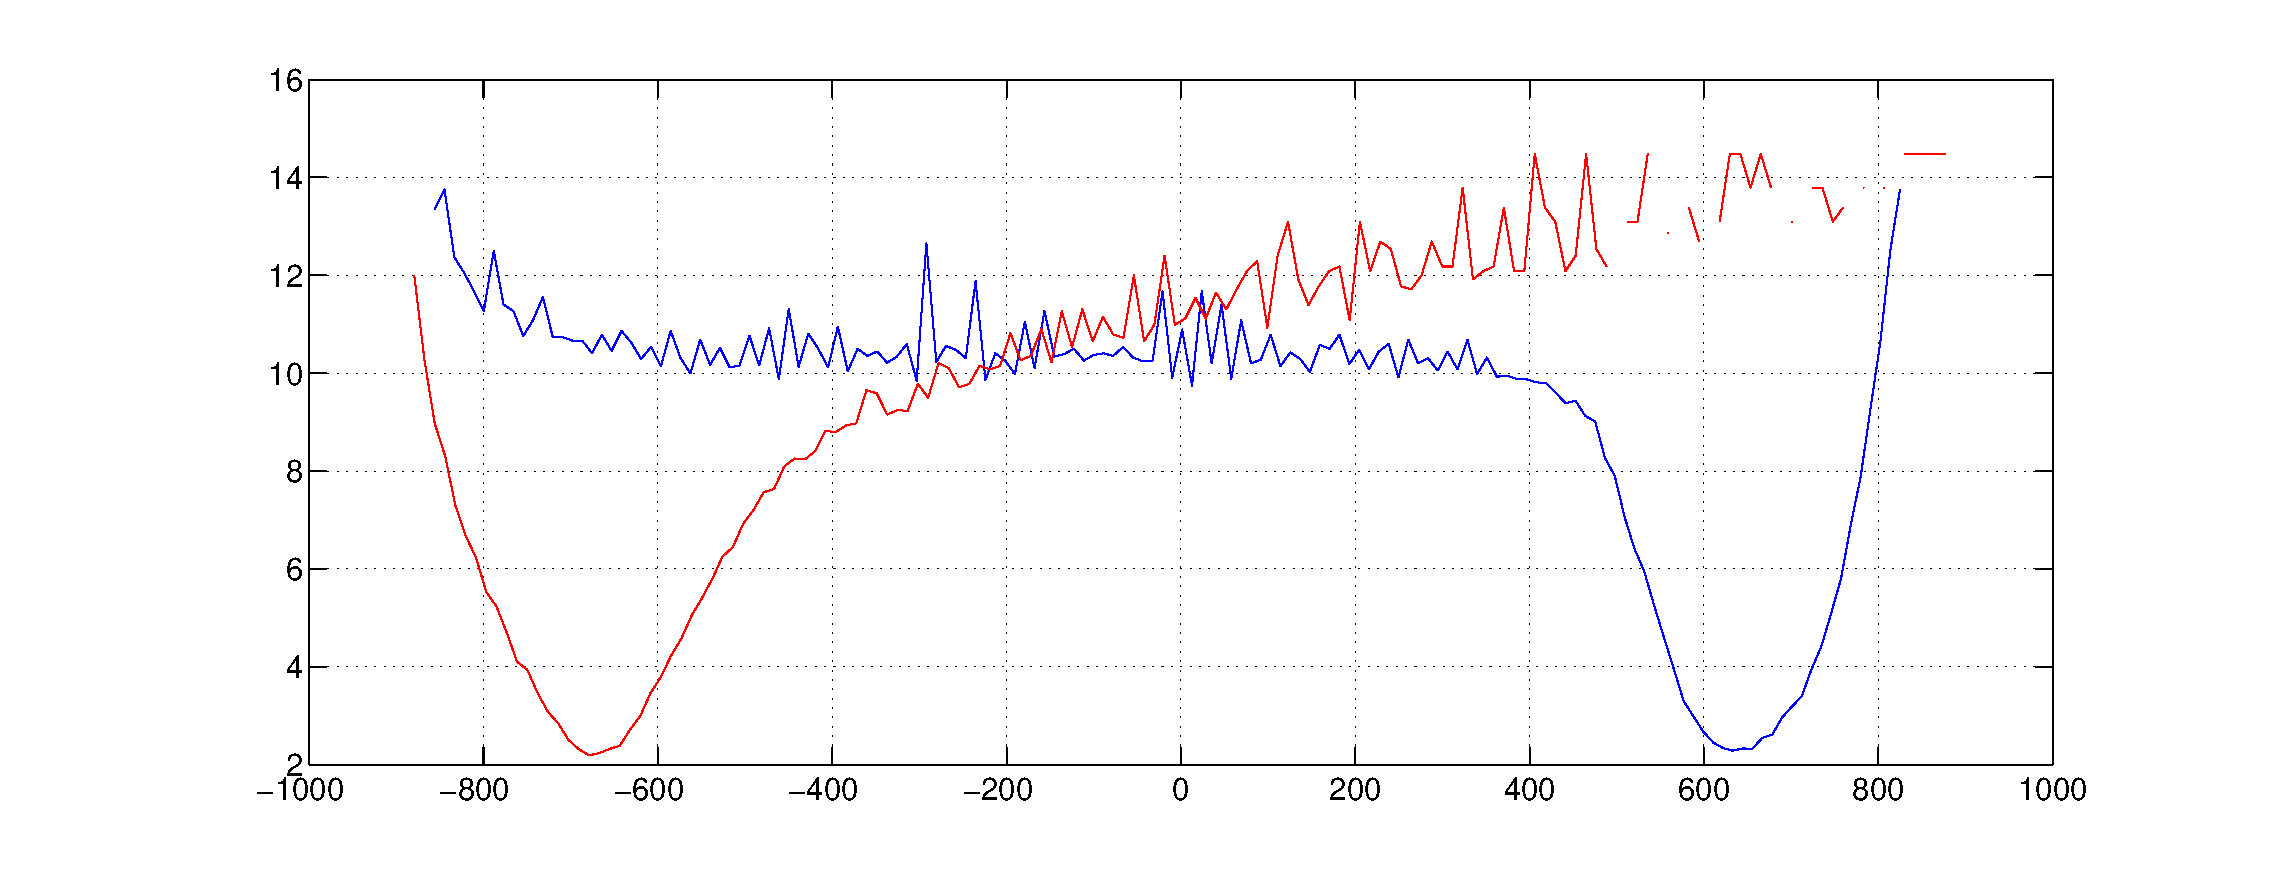
\includegraphics[height=5cm,width=12cm]{both_wells_I1_5k_700_3and4.eps}
  %  \caption{Applying step fitting to bead trace}
    \label{fig:graph11}
\end{figure}


\end{frame}
%%-----------------------------------------------------------------------
\begin{frame}{Single well- I900, 700, both, 6, 3} 
SD = 286.6 nm , Depth = 2.7 $K_BT$ ; bead is lost at this low intensity\\
\begin{figure}
    \centering
    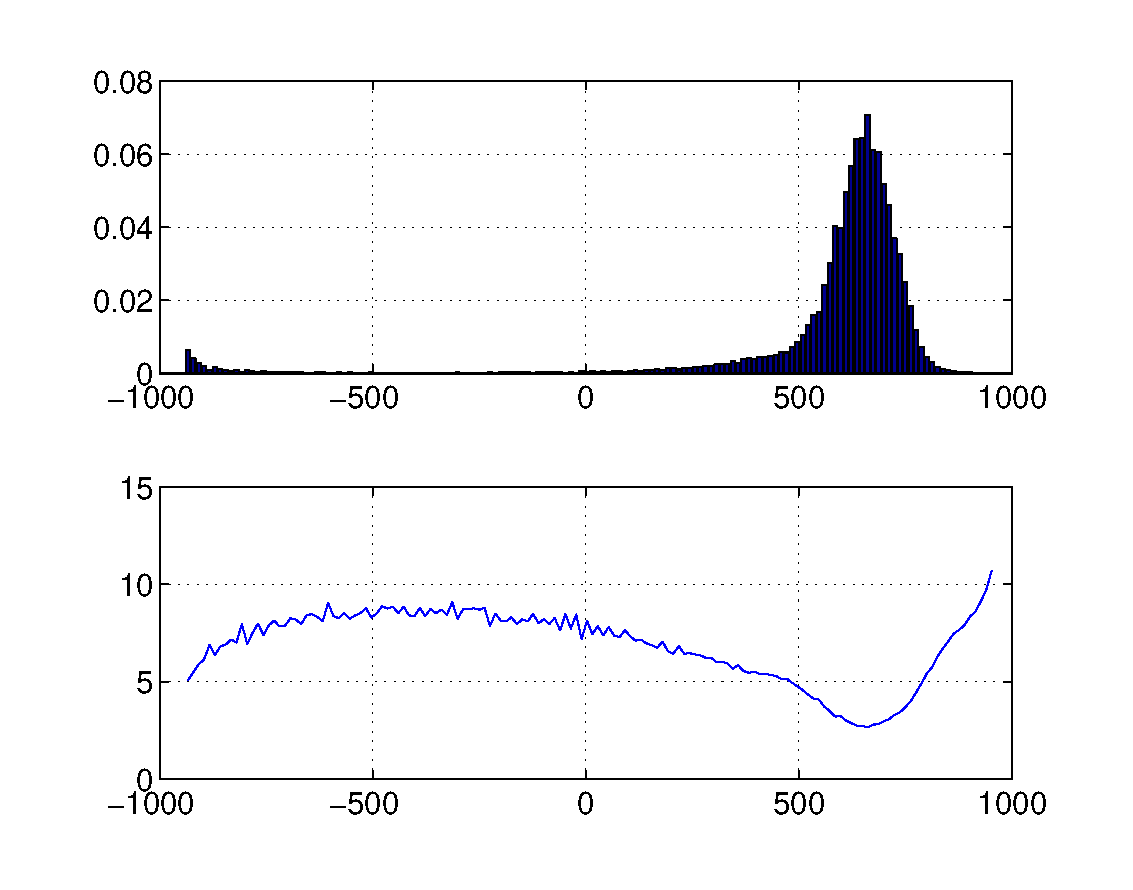
\includegraphics[height=5cm,width=12cm]{right_well_I900_1.eps}
 %   \caption{Applying step fitting to bead trace}
    \label{fig:graph12}
\end{figure}


\end{frame}

%%-----------------------------------------------------------------------
\begin{frame}{Shift to 6,3 ; I4k, 700, both, 6, 3} 
R=3.2 $K_BT$, SD = 48.3 nm, L = 3.4 $K_BT$, SD = 37.1 nm 
\begin{figure}
    \centering
    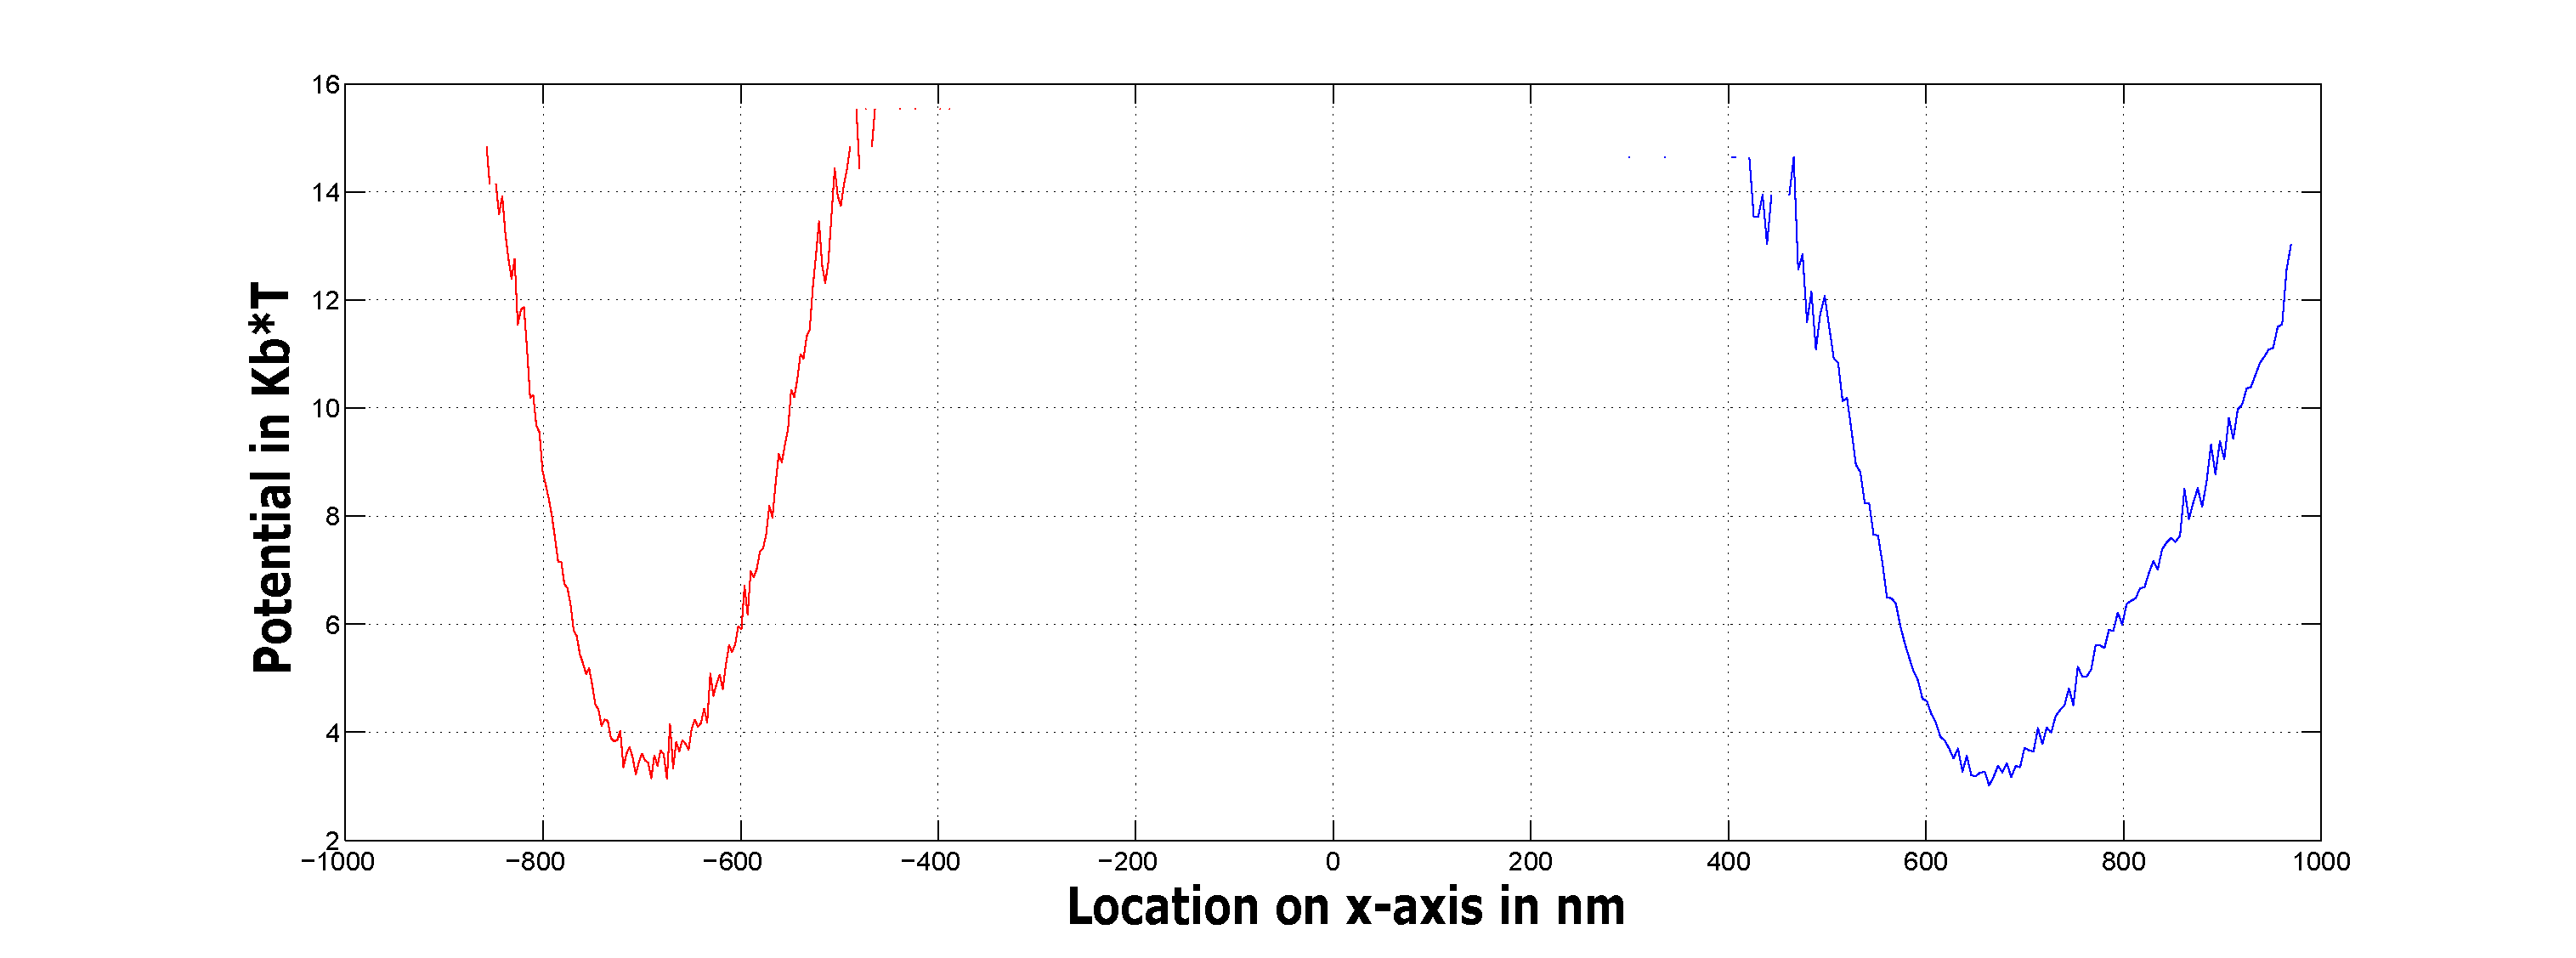
\includegraphics[height=5cm,width=12cm]{I4k_both_wells_700_1.eps}
 %   \caption{Applying step fitting to bead trace}
    \label{fig:graph13}
\end{figure}


\end{frame}

%%-----------------------------------------------------------------------
\begin{frame}{Shift to 6,3 ; I4k, 700, both, 6, 3} 
R=2.6 $K_BT$, SD = 67.7 nm, L = 3.25 $K_BT$, SD = 37.3 nm 
\begin{figure}
    \centering
    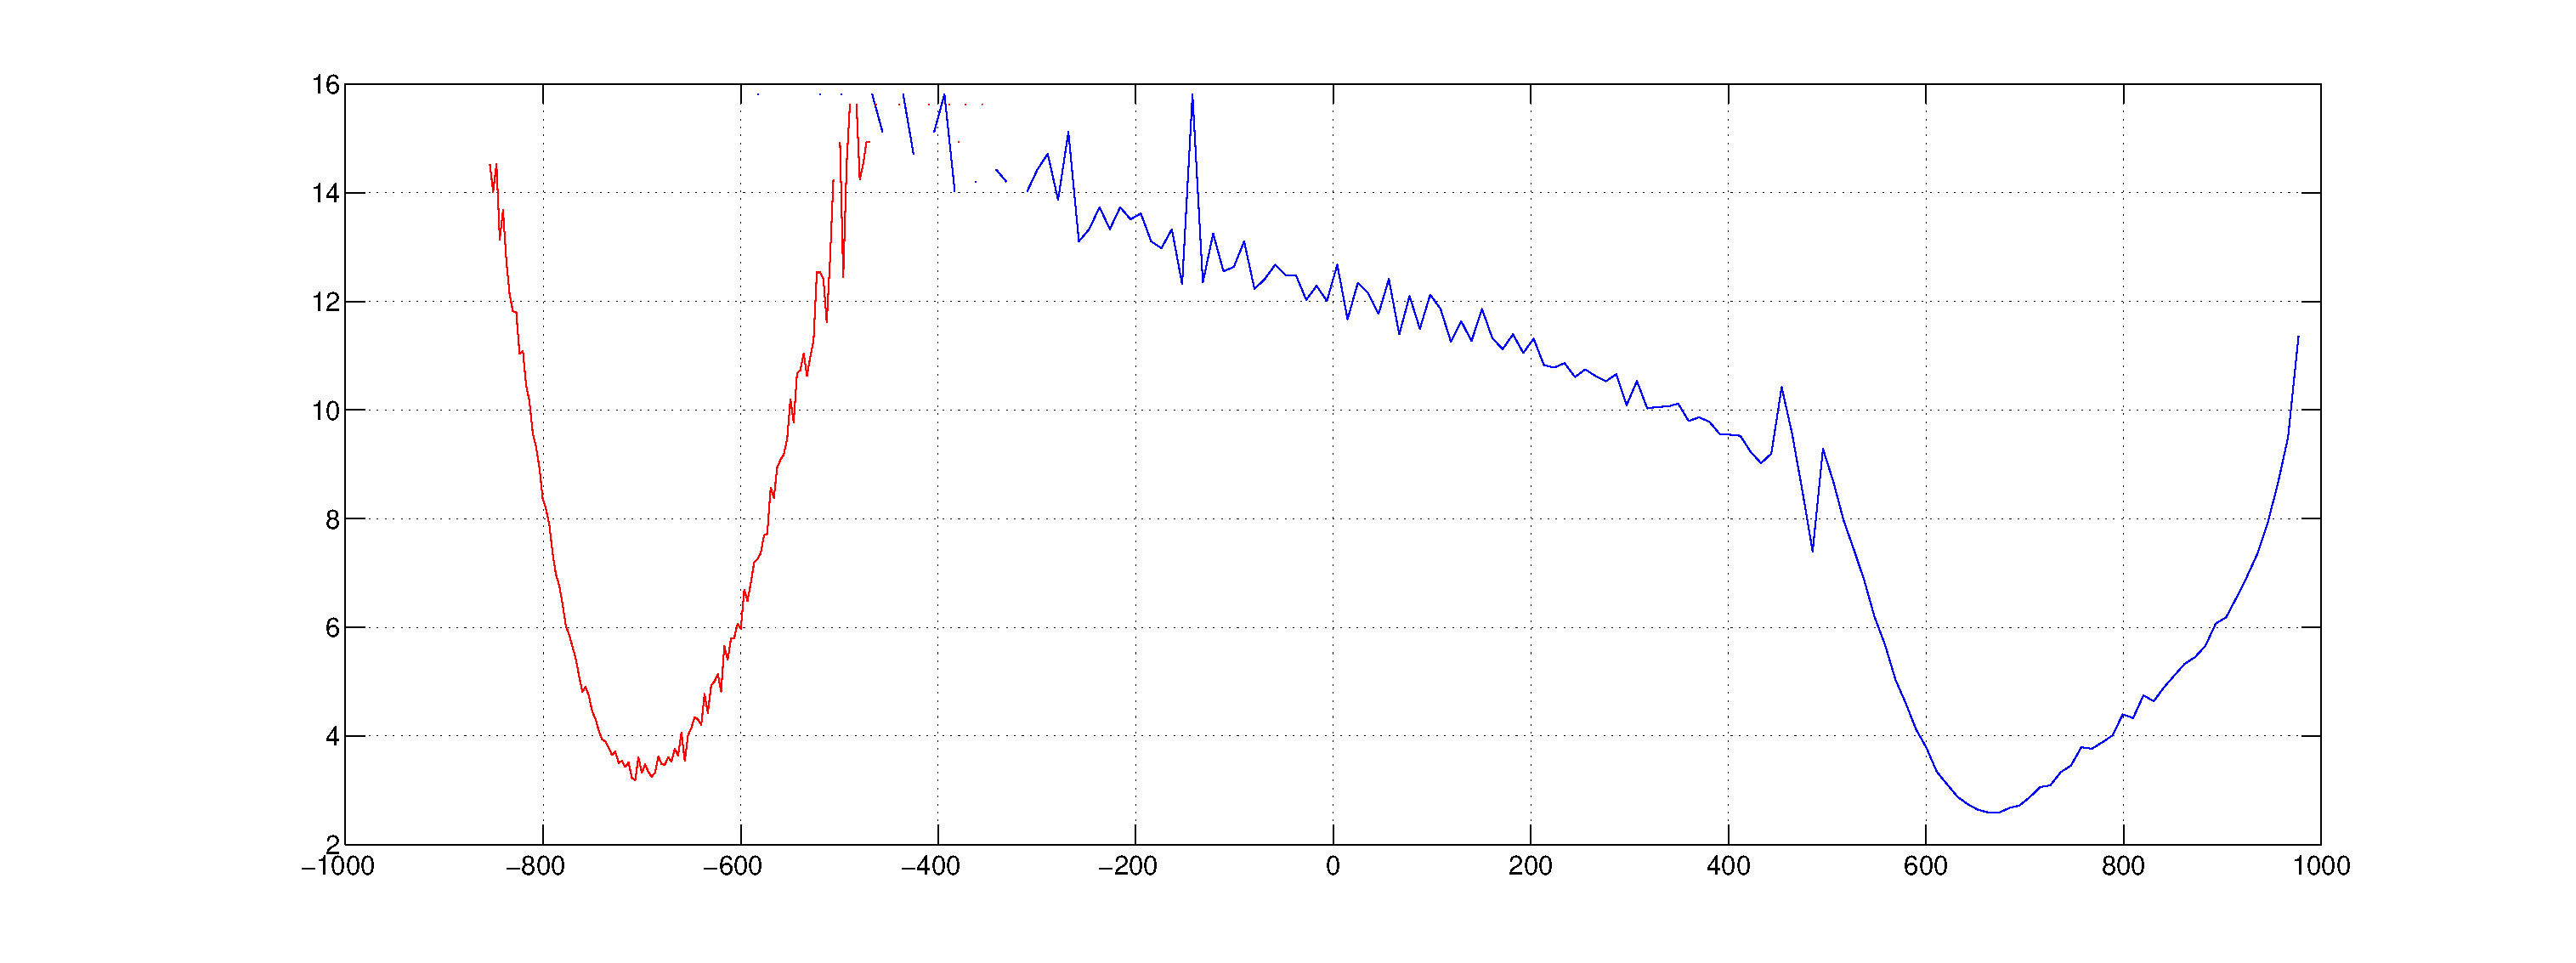
\includegraphics[height=5cm,width=12cm]{I4k_both_wells_700_2.eps}
 %   \caption{Applying step fitting to bead trace}
    \label{fig:graph14}
\end{figure}


\end{frame}
%%-----------------------------------------------------------------------
\section{Low intensity wells}
\begin{frame}{I900, 700, 6, 3, Left} 
Wide well, 4 $K_BT$, SD = 126.23 nm \\$\rightarrow$ Most beads lost at this intensity from left
\begin{figure}
    \centering
    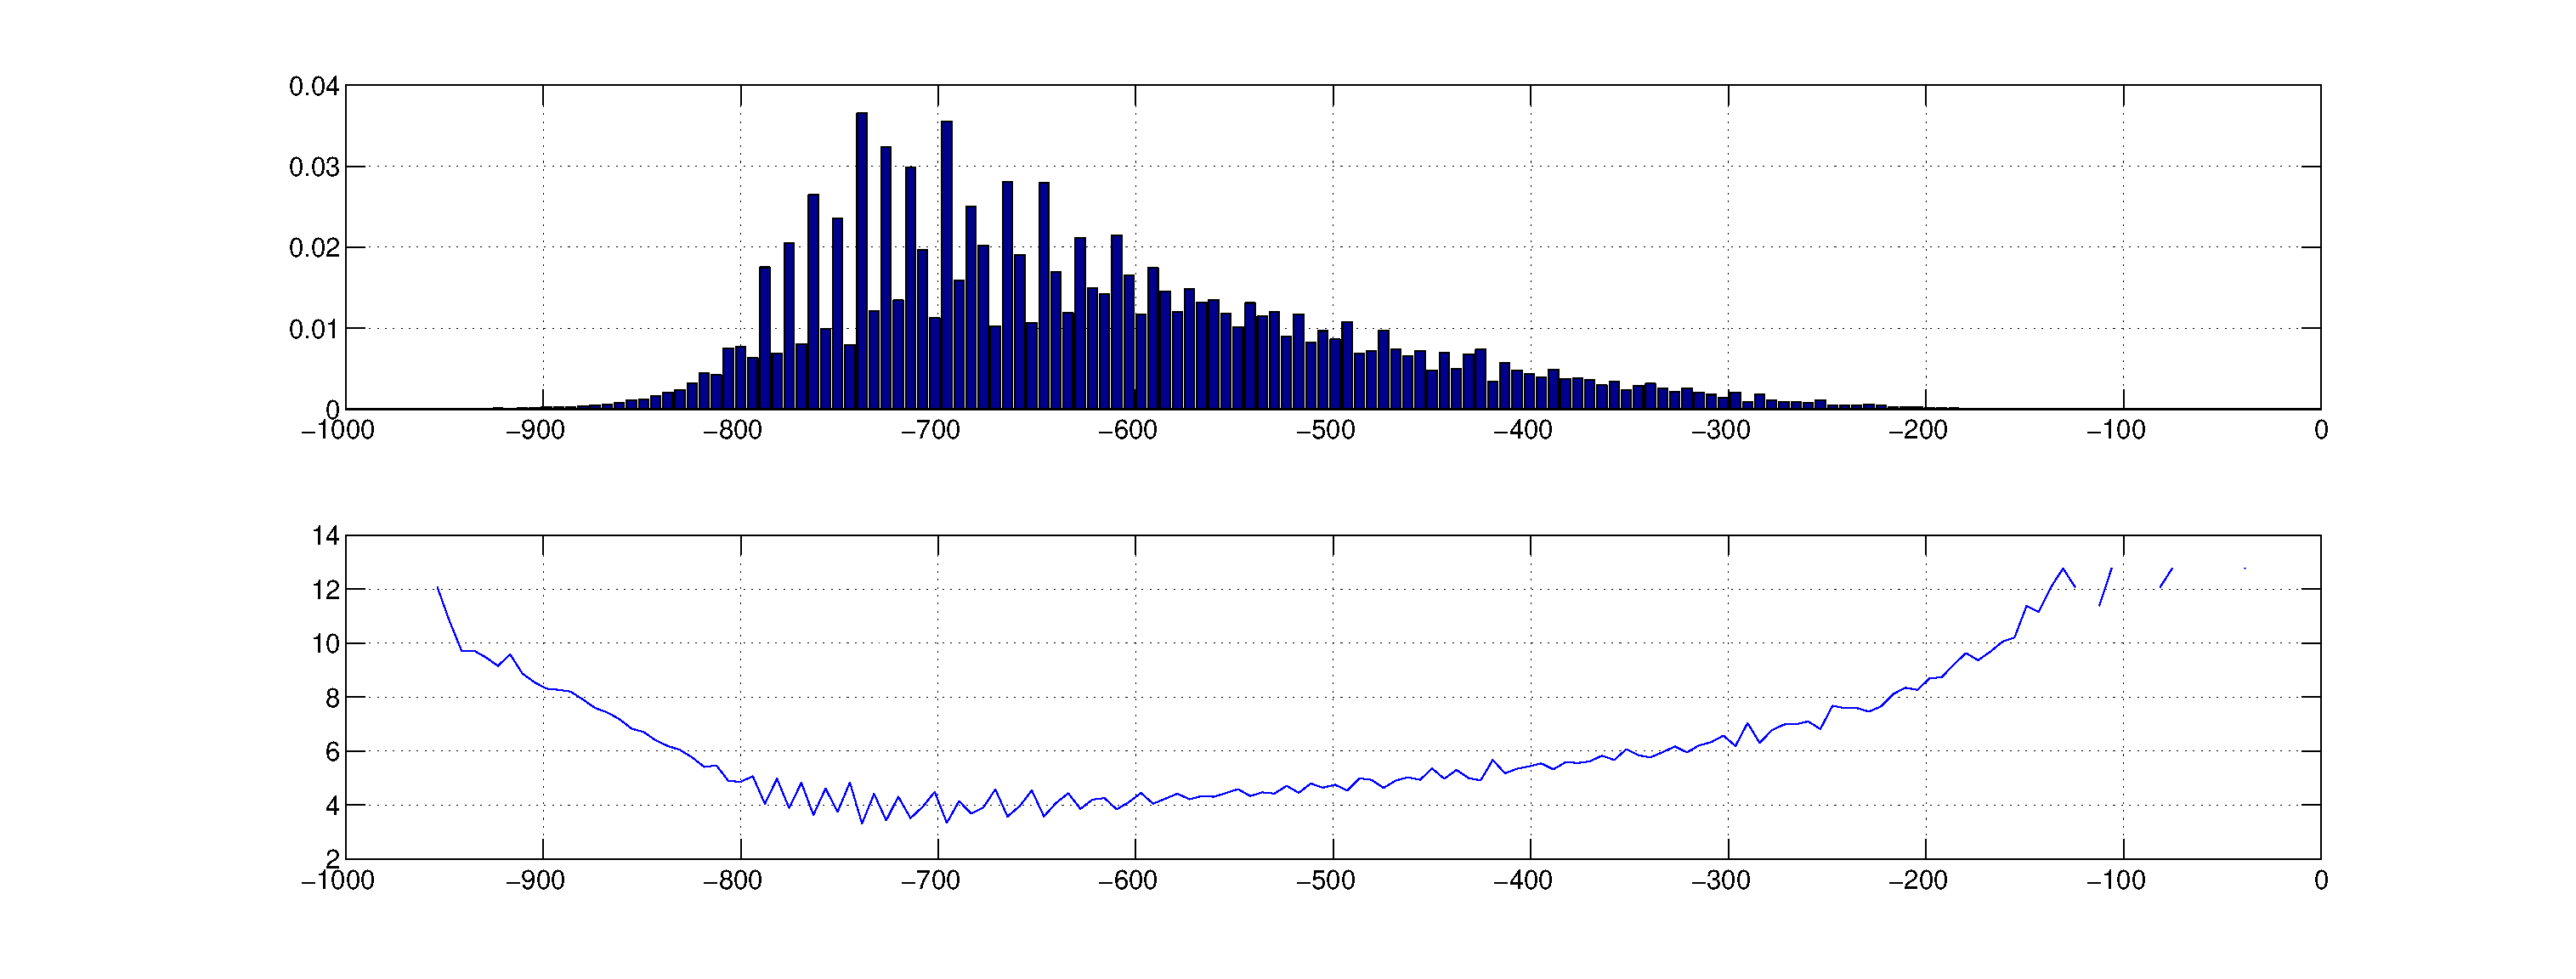
\includegraphics[height=5cm,width=12cm]{I900_left_1.eps}
 %   \caption{Applying step fitting to bead trace}
    \label{fig:graph15}
\end{figure}


\end{frame}

%%-----------------------------------------------------------------------

\begin{frame}{I900, 700, 6, 3, Left} 
Wide well, 3.6 $K_BT$, SD = 78.35 nm \\$\rightarrow$ Most beads lost at this intensity from left
\begin{figure}
    \centering
    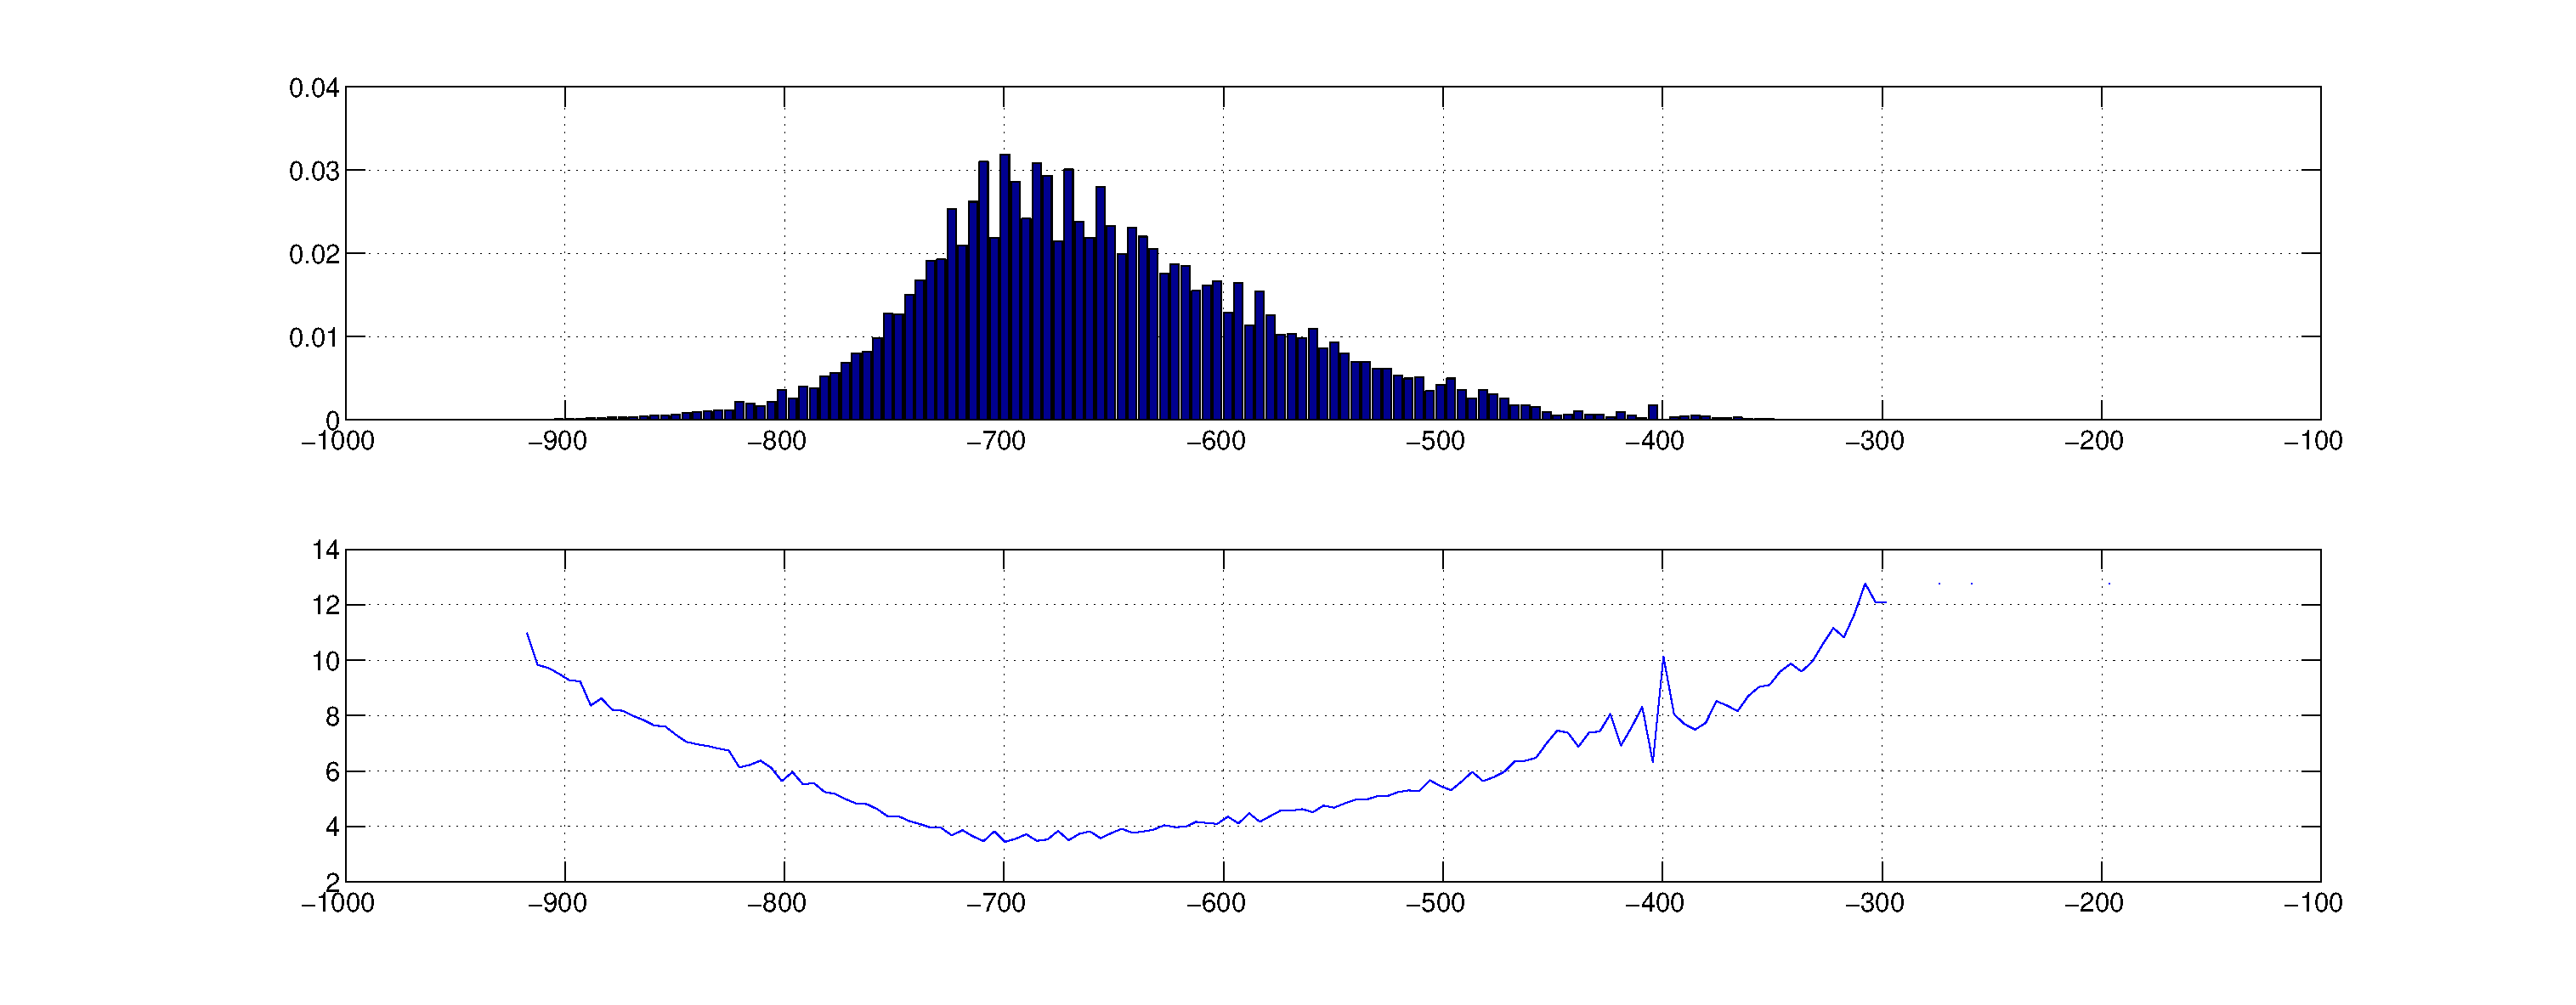
\includegraphics[height=5cm,width=12cm]{I900_left_3.eps}
 %   \caption{Applying step fitting to bead trace}
    \label{fig:graph16}
\end{figure}


\end{frame}

%%-----------------------------------------------------------------------
\begin{frame}{I900, 700, 6, 3, Right} 
Wide well, 2.85 $K_BT$, SD = 142 nm \\$\rightarrow$ Bead is lost at this intensity but bead transition to left probable
\begin{figure}
    \centering
    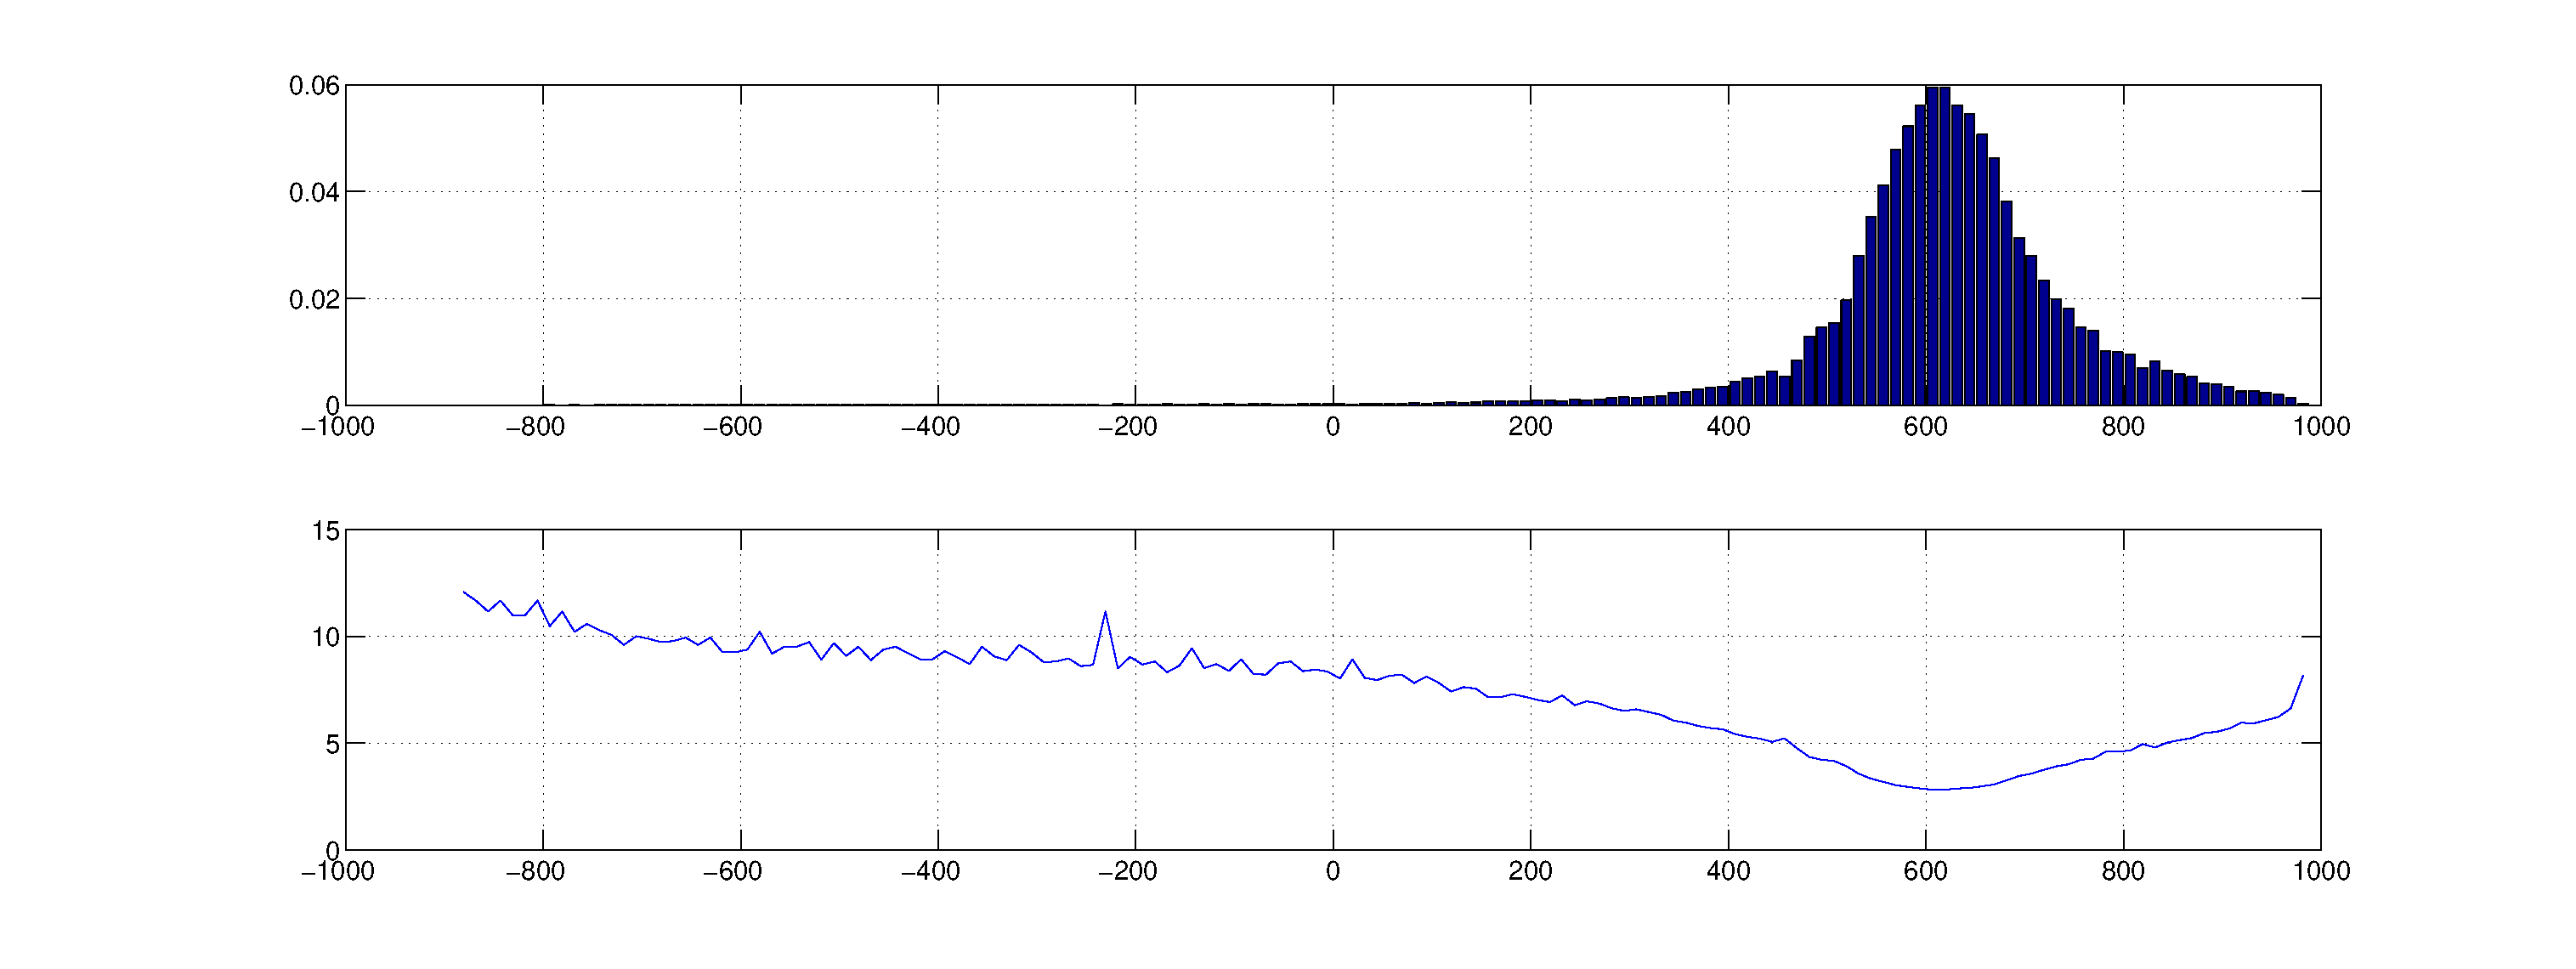
\includegraphics[height=4.5cm,width=12cm]{I900_both_1.eps}
 %   \caption{Applying step fitting to bead trace}
    \label{fig:graph17}
\end{figure}


\end{frame}

%%-----------------------------------------------------------------------
\begin{frame}{I900, 700, 6, 3, Right} 
Wide well, 2.8 $K_BT$ \\$\rightarrow$ Bead is lost at this intensity but bead transition to left probable
\begin{figure}
    \centering
    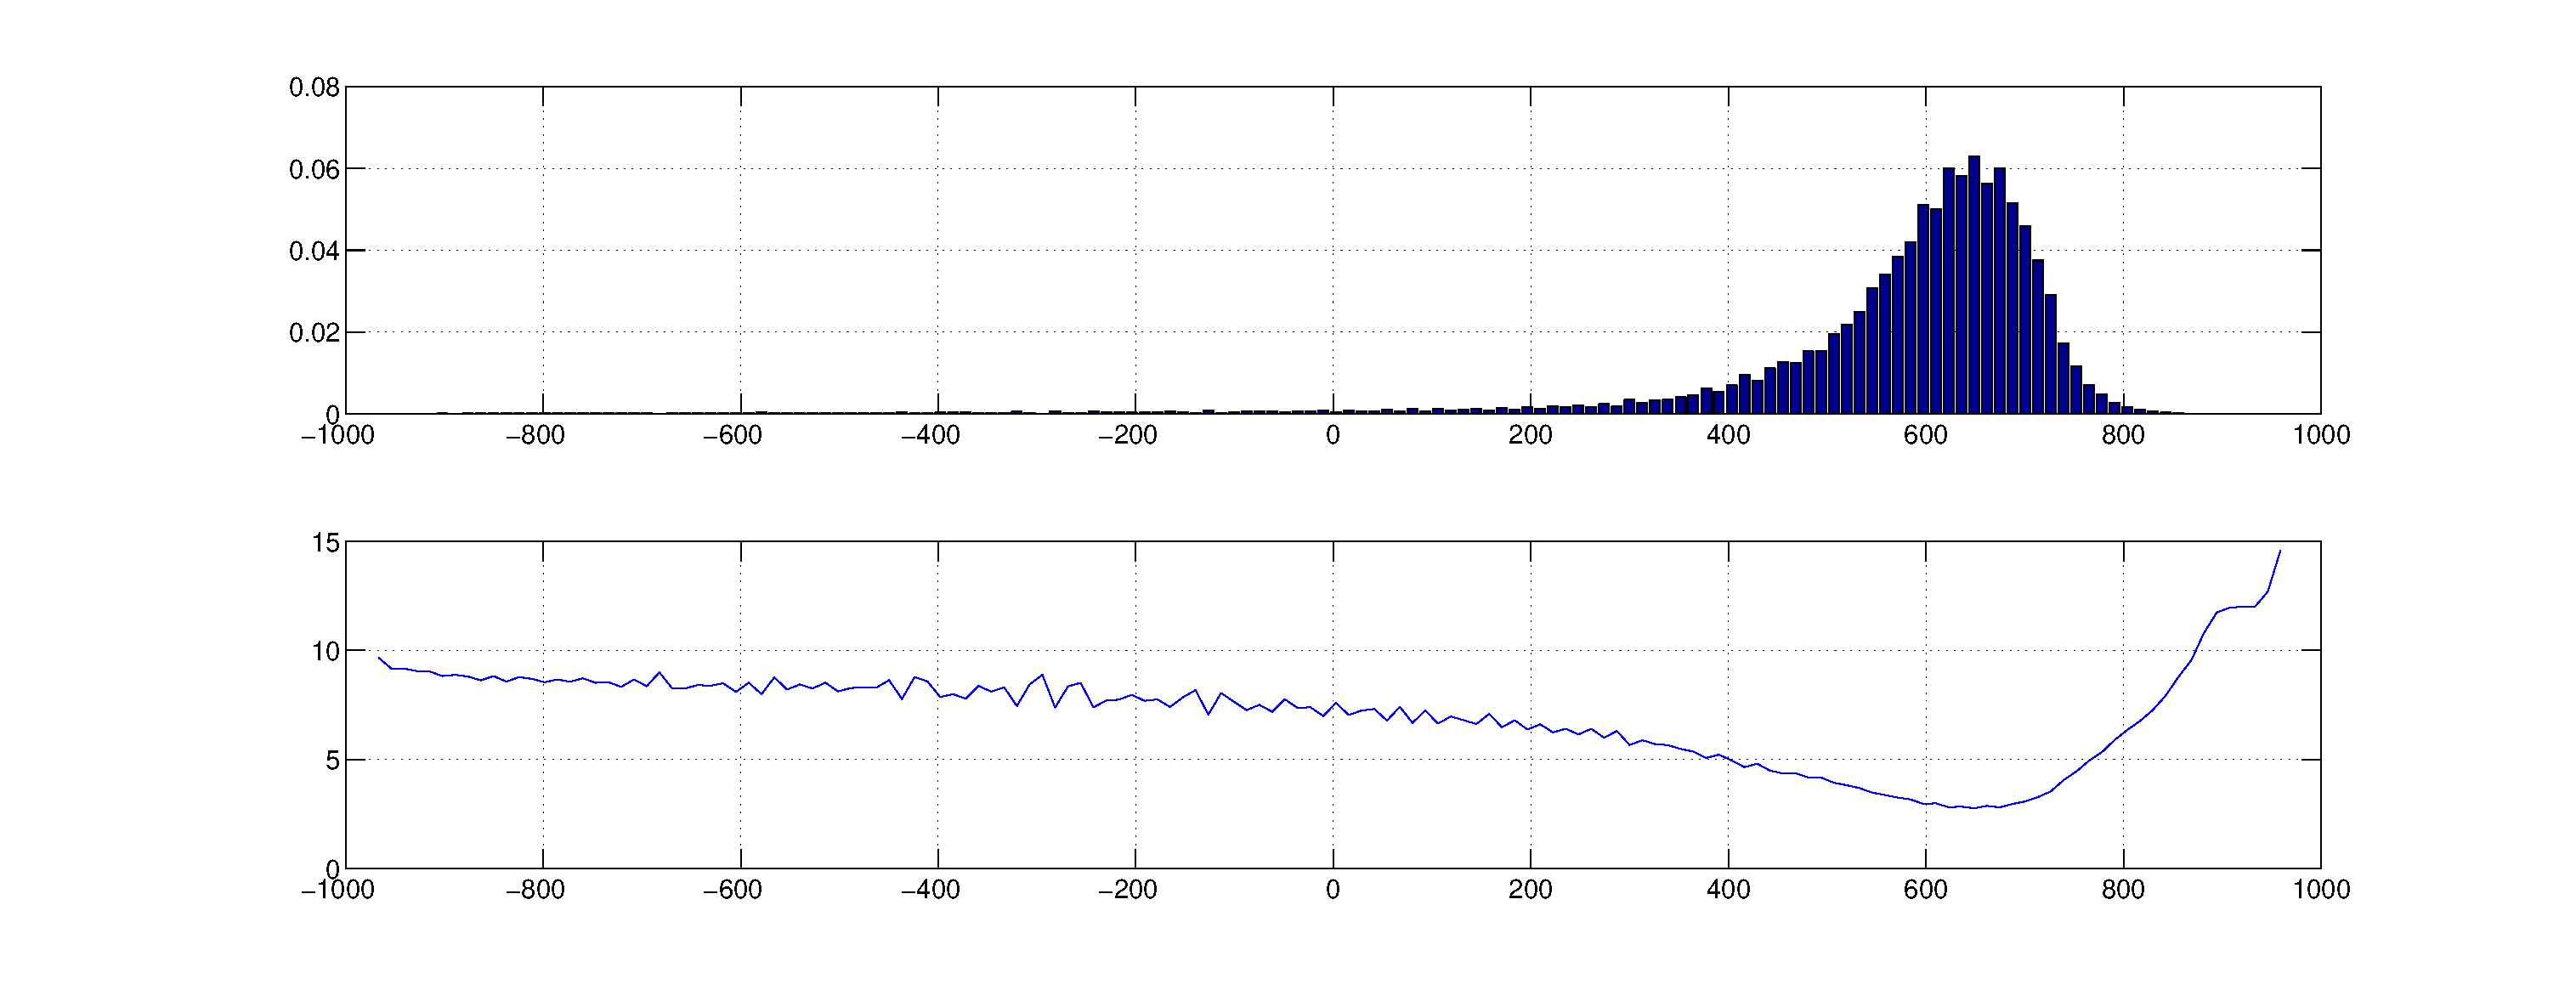
\includegraphics[height=4.5cm,width=12cm]{I900_right_16.eps}
 %   \caption{Applying step fitting to bead trace}
    \label{fig:graph18}
\end{figure}


\end{frame}

%%-----------------------------------------------------------------------
\begin{frame}{I900, 700, 6, 3, Right} 
Wide well, 2.9 $K_BT$ (values near -1000 not trustworthy, neural nw issues)$\rightarrow$ Bead is lost at this intensity but bead transition to left probable
\begin{figure}
    \centering
    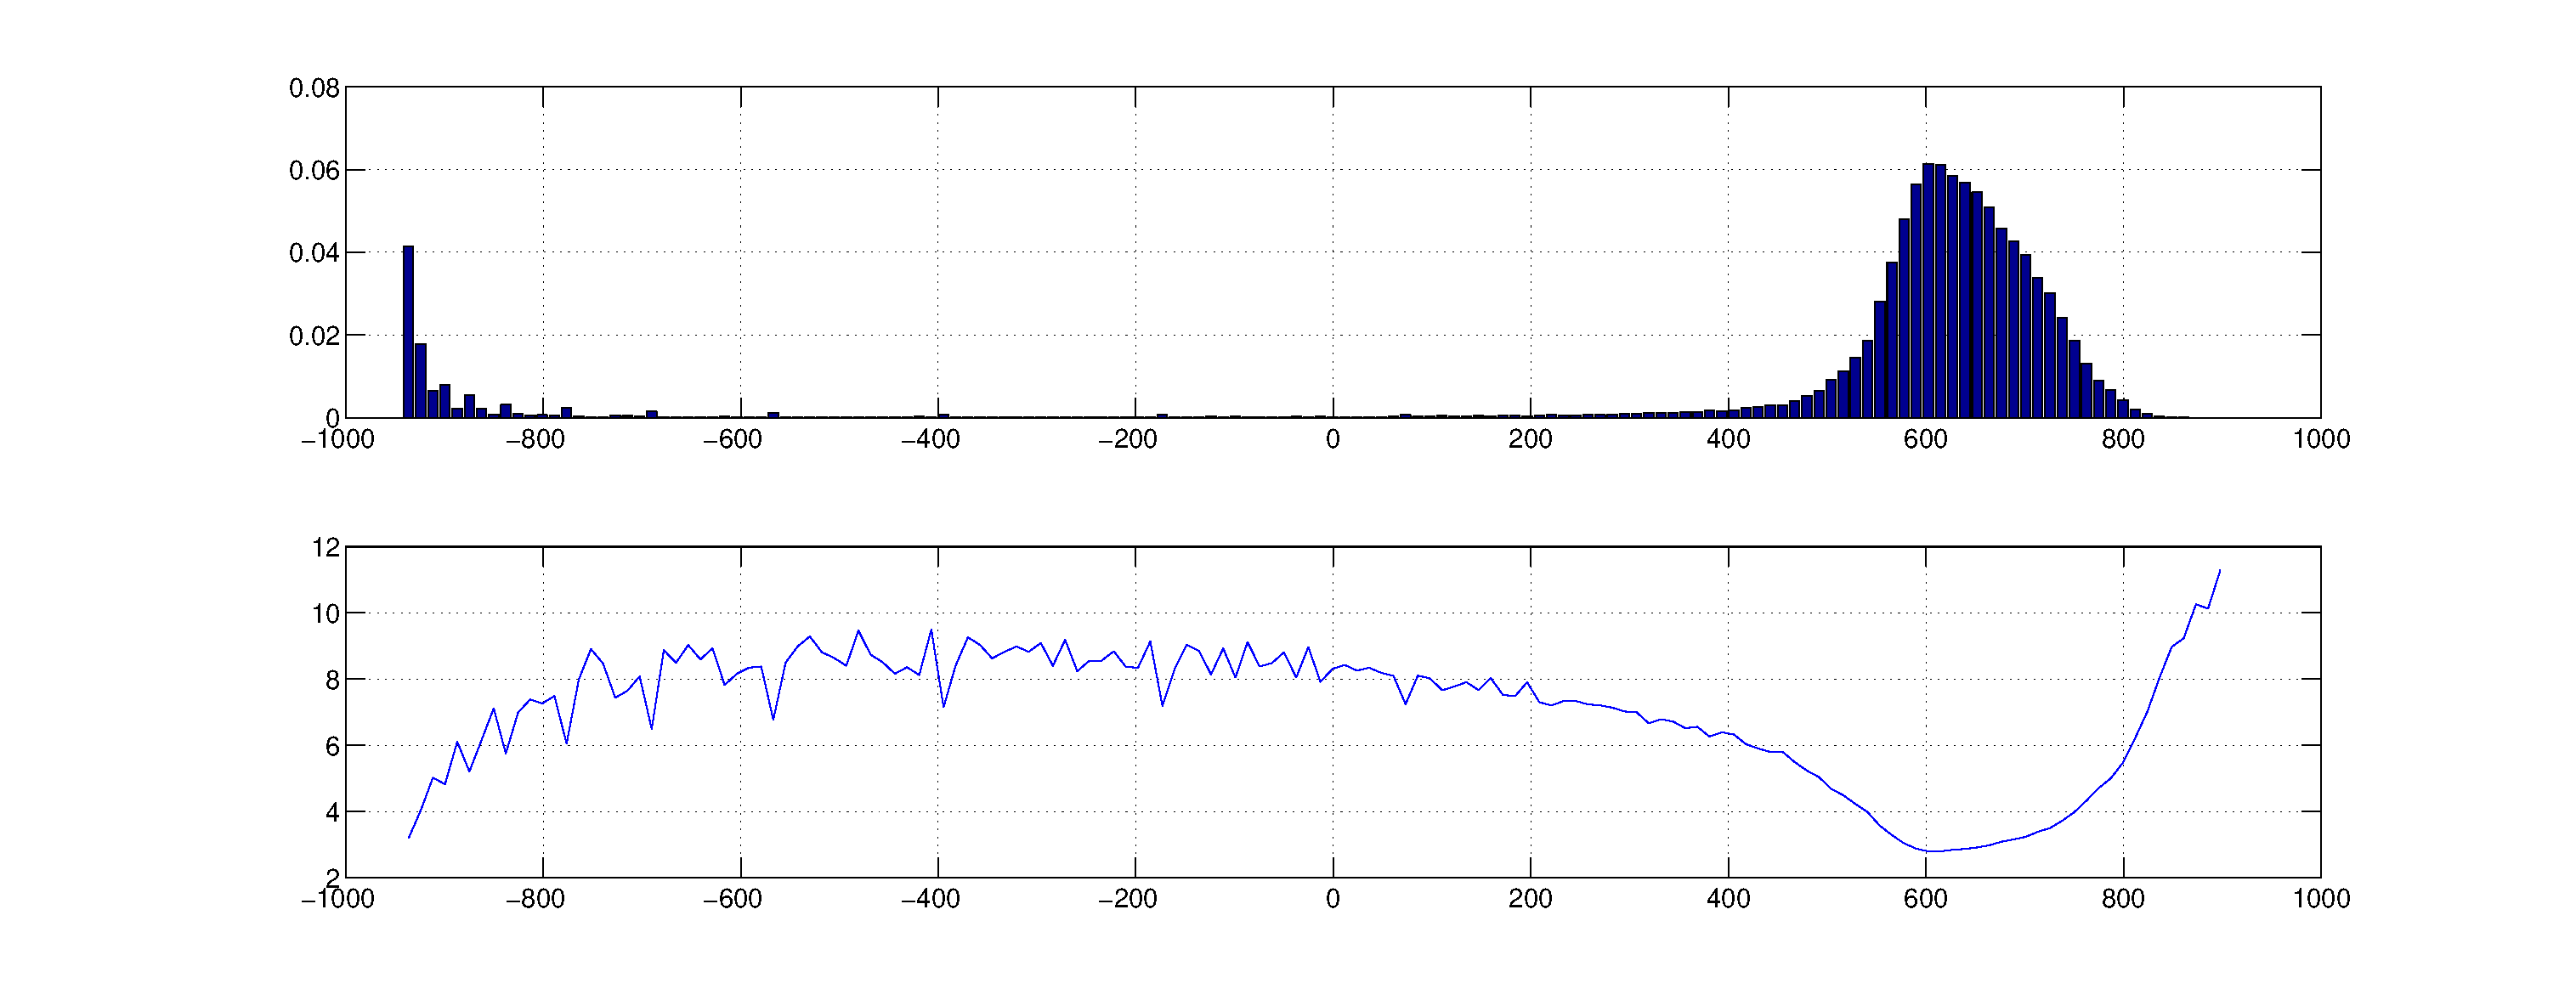
\includegraphics[height=4.5cm,width=12cm]{I900_both_2.eps}
 %   \caption{Applying step fitting to bead trace}
    \label{fig:graph19}
\end{figure}


\end{frame}

%%-----------------------------------------------------------------------
\begin{frame}{I900, 700, 6, 3, Right} 
R= 3.15 $K_BT$, L = 4.55 $K_BT$, Height = 7.5$K_BT$, Total SD = 552.67 nm $\rightarrow$ Bead is lost, transition seen for small amount of time
\begin{figure}
    \centering
    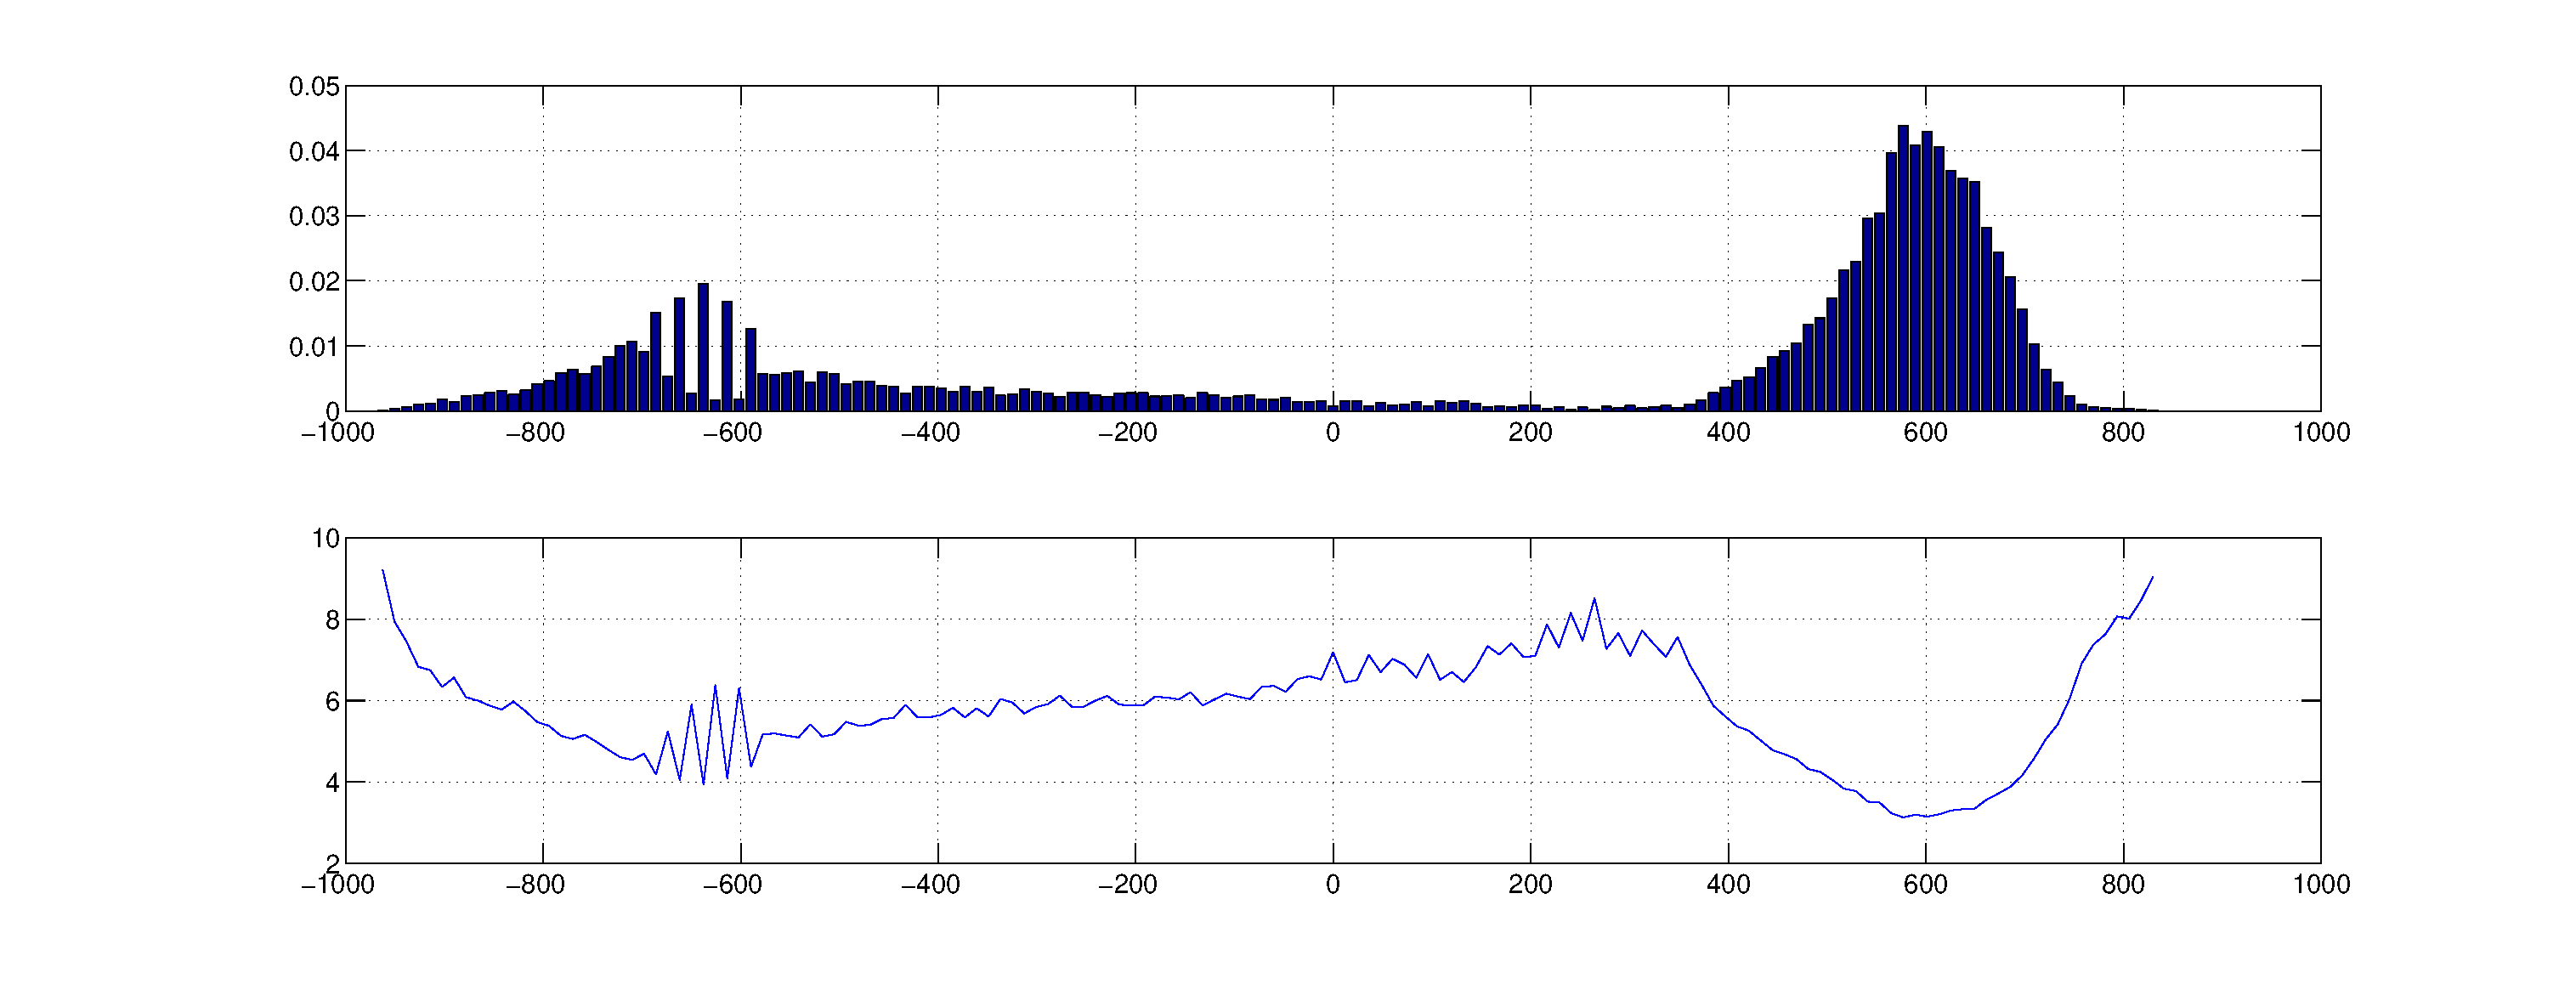
\includegraphics[height=4.5cm,width=12cm]{I900_right_15.eps}
 %   \caption{Applying step fitting to bead trace}
    \label{fig:graph20}
\end{figure}


\end{frame}

%%-----------------------------------------------------------------------
\begin{frame}{I900, 700, 6, 3, Right} 
R= 4 $K_BT$, L(not so good) = 4.5 $K_BT$, Height = 6.5$K_BT$, Total SD = 600 nm $\rightarrow$ Bead is lost, transition seen for small amount of time
\begin{figure}
    \centering
    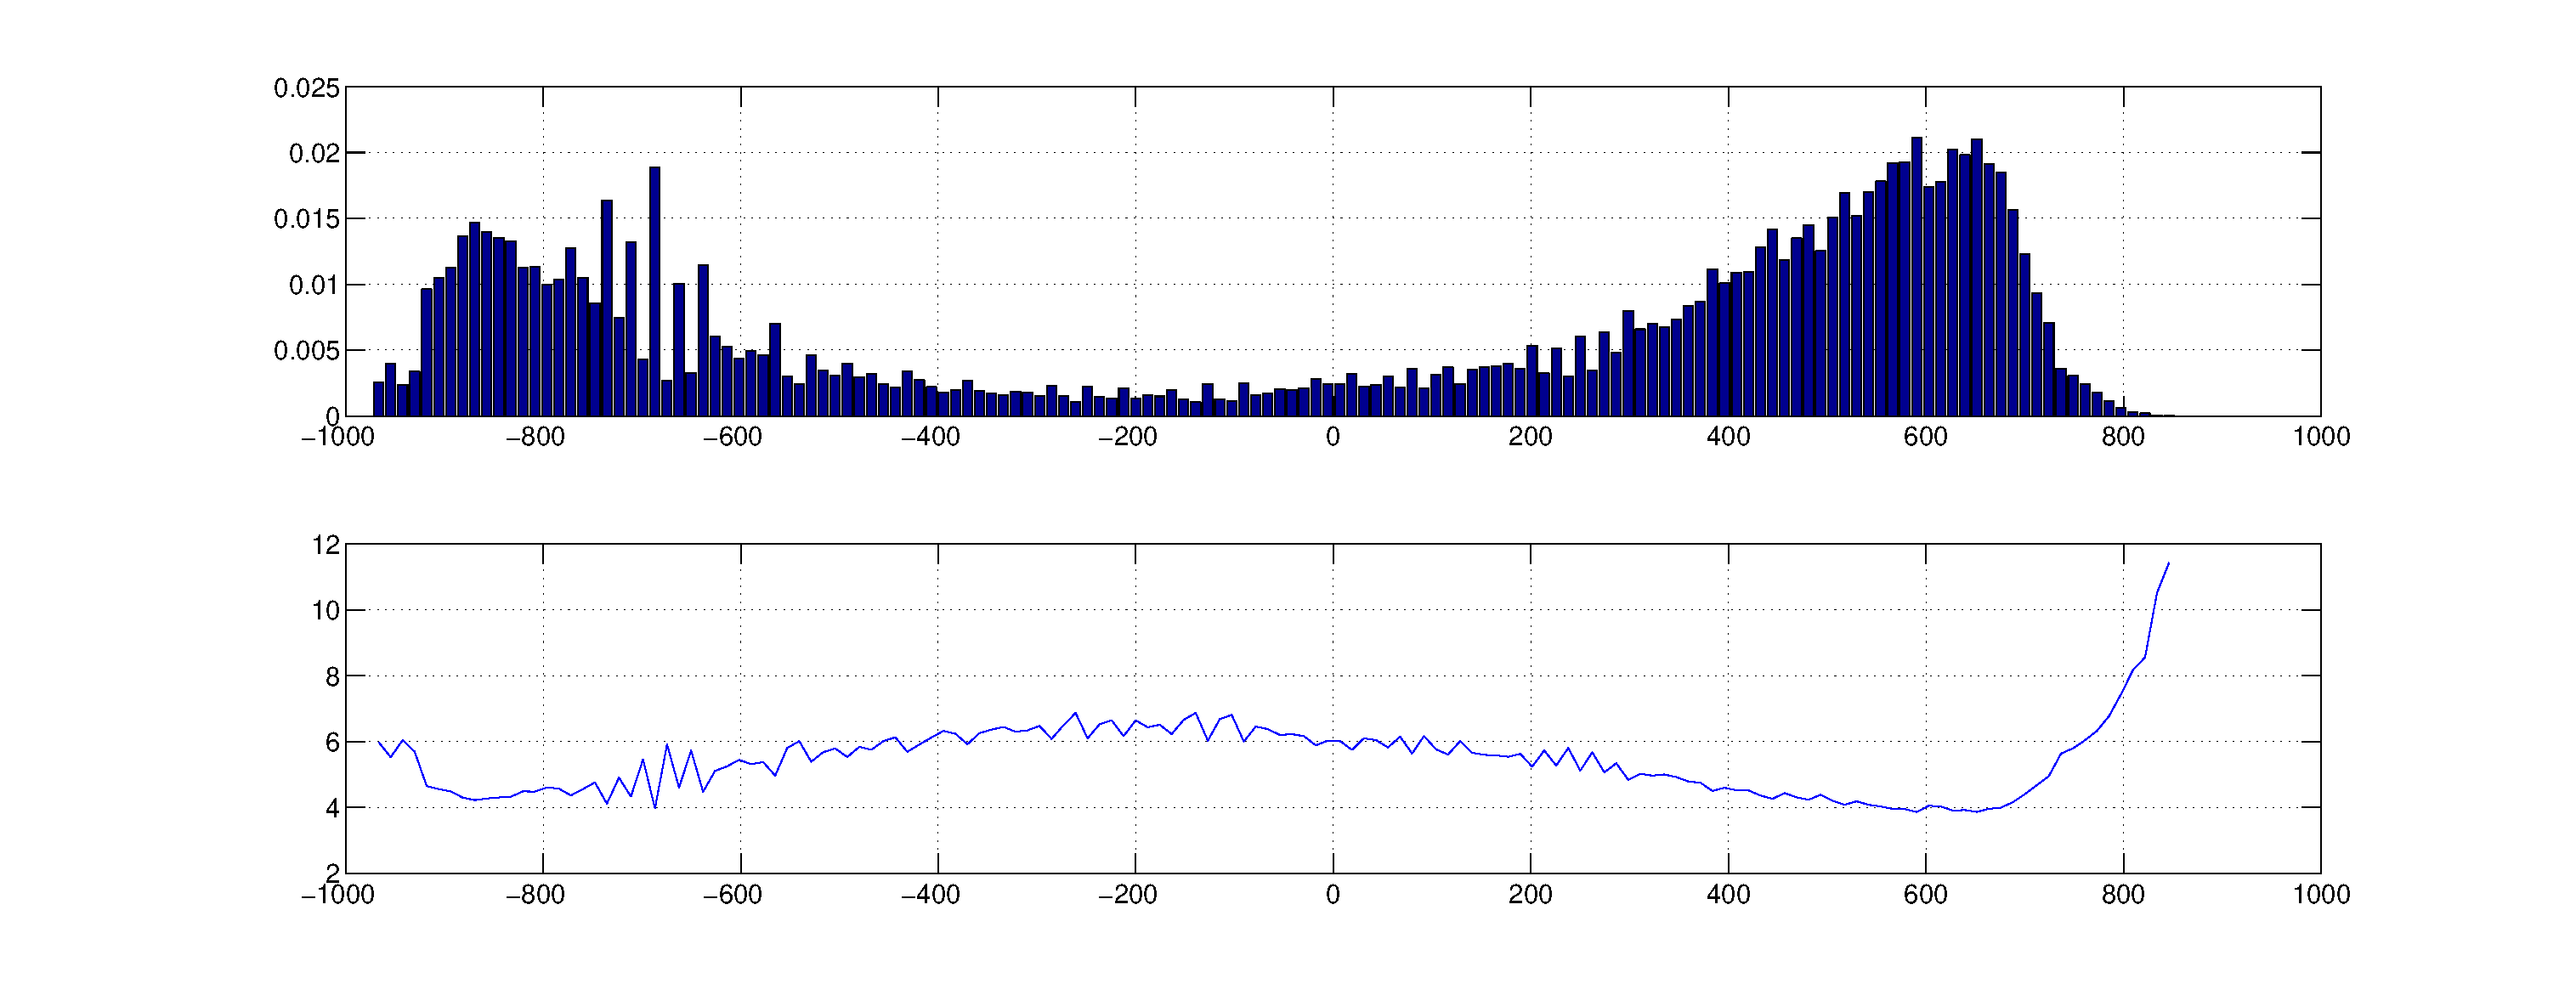
\includegraphics[height=4.5cm,width=12cm]{I900_right_20.eps}
 %   \caption{Applying step fitting to bead trace}
    \label{fig:graph21}
\end{figure}


\end{frame}

%%-----------------------------------------------------------------------
\begin{frame}{I800, 700, 6, 3, Right} 
R= 3.6 $K_BT$, L(not so good) = 4.5 $K_BT$, Height = 6.5$K_BT$, Total SD = 633.58 nm $\rightarrow$ Bead is almost always lost, transition seen for small amount of time
\begin{figure}
    \centering
    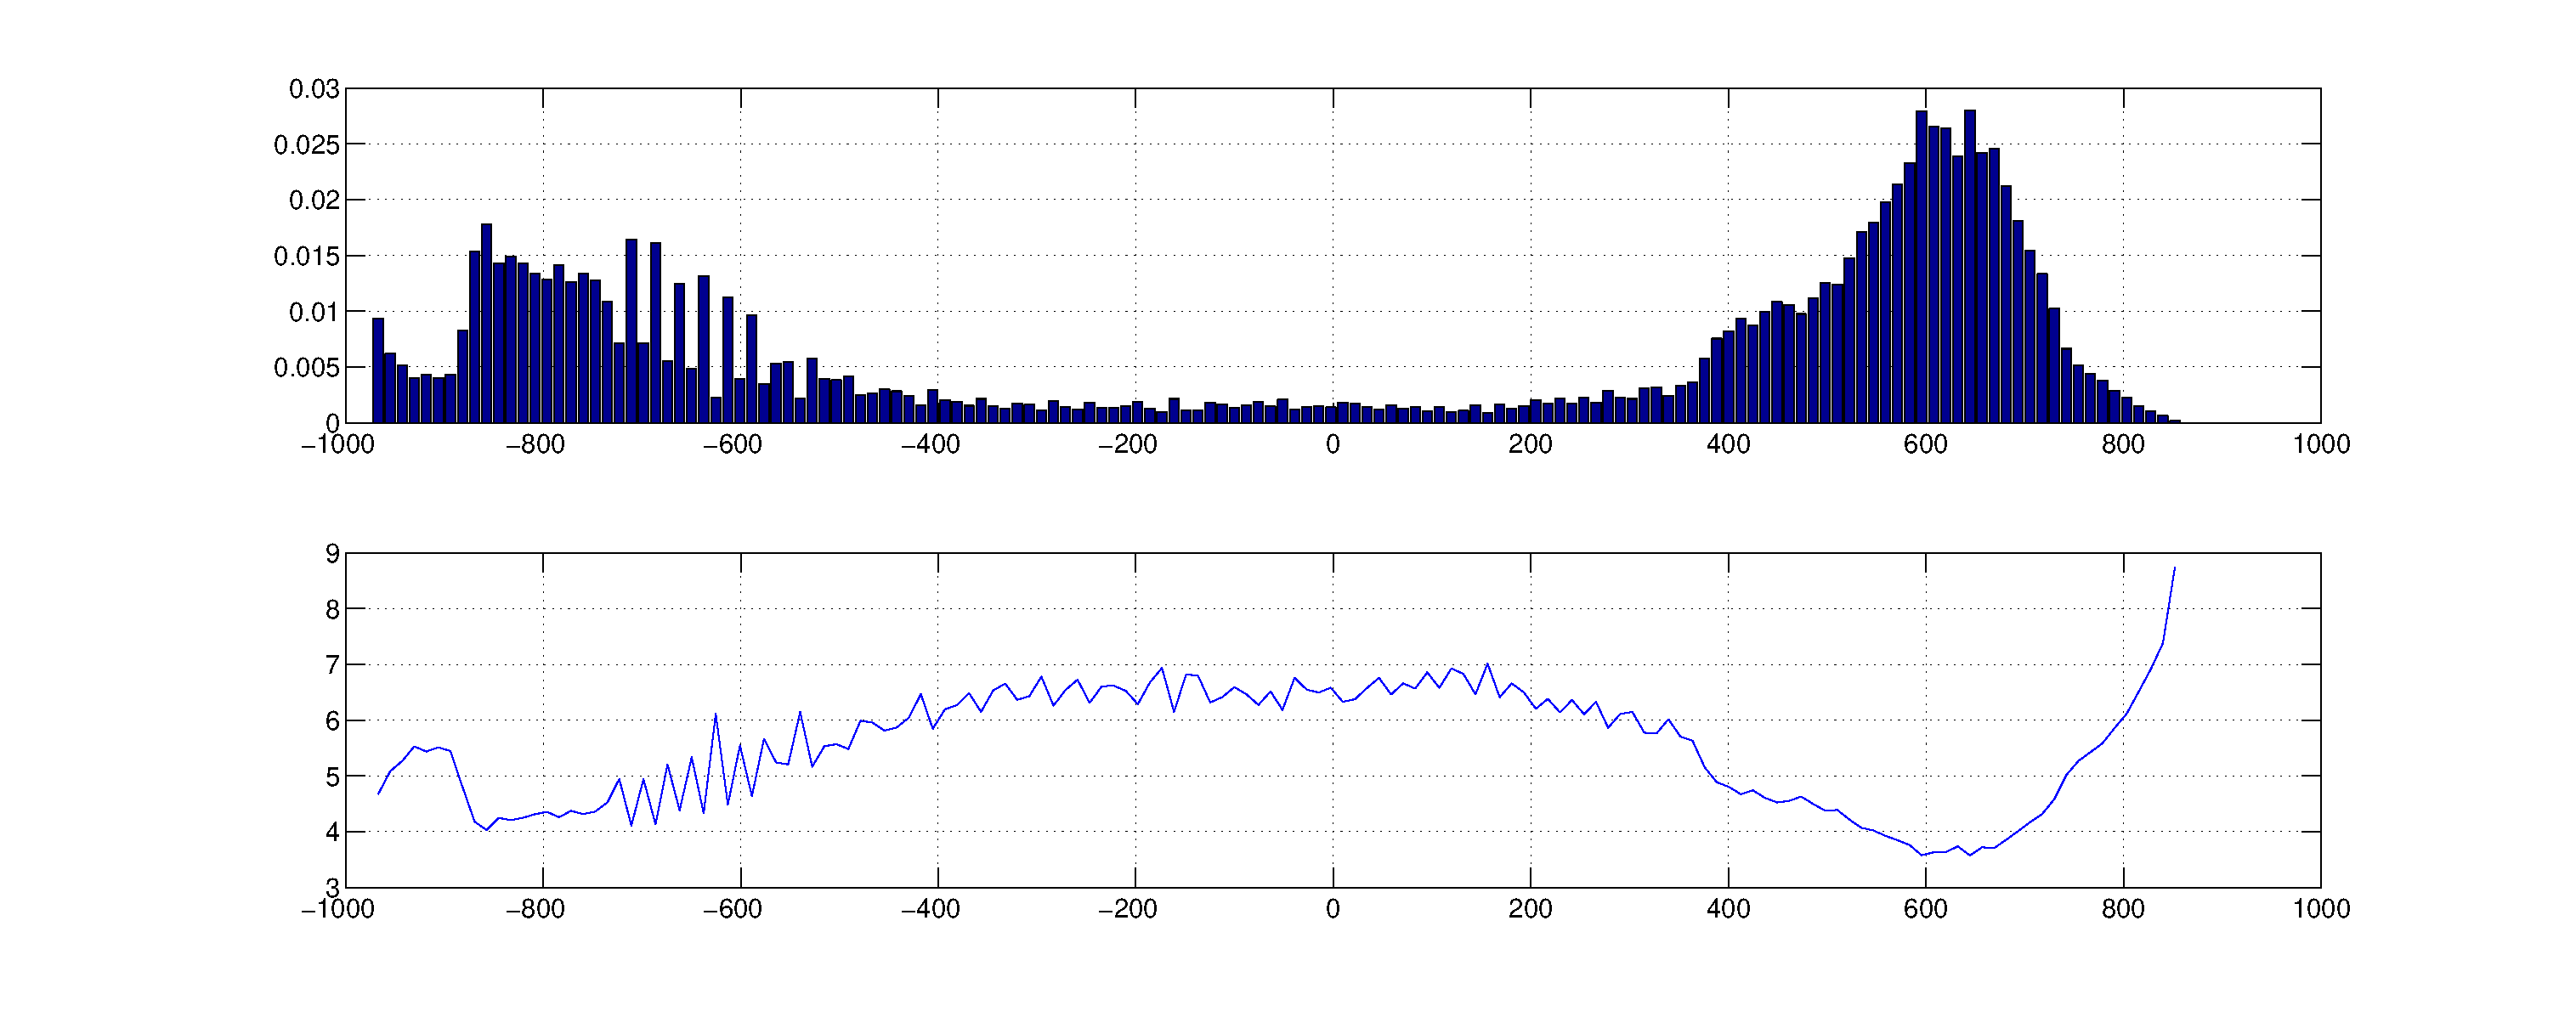
\includegraphics[height=4.5cm,width=12cm]{I800_right_1.eps}
 %   \caption{Applying step fitting to bead trace}
    \label{fig:graph22}
\end{figure}


\end{frame}

%%-----------------------------------------------------------------------
\section{Transition by tilting wells}
\begin{frame}{Idea} 

\begin{itemize}

\item For low intensities, a few instances of transition from one well to other is seen
\item So barrier is lowered enough for bead transition to occur
\item However, the bead is almost always lost
\item How about transition at higher intensities by tilting the wells ?
\item Possible by modulating the on time of the multiplexing of trapping beam at the two locations -700 and +700

\end{itemize}


\end{frame}

%%-----------------------------------------------------------------------
\begin{frame}{Process of transition from Right to Left} 

\begin{itemize}

\item Trap bead at +700; potential well formed at +700, 4 blinks to L and R each, each blink for 20 $\mu s$
\item Modulate the on times as :
\end{itemize}
\begin{center} 
\begin{tabular}{| l | c | r |} 
\hline Total & Left & Right \\ 
\hline 8 & 4 & 4 \\ 
\hline 8 & 5 & 3 \\ 
\hline 8 & 6 & 2 \\ 
\hline 8 & 7 & 1 \\ 
\hline \hline 8 & 4 & 4 \\ 
\hline \end{tabular} 
\end{center}

\end{frame}

%%-----------------------------------------------------------------------
\begin{frame}{Transition as photodiode O/P} 
Bead transfer happens at L=6 ,R=2 blinks
\begin{figure}
    \centering
    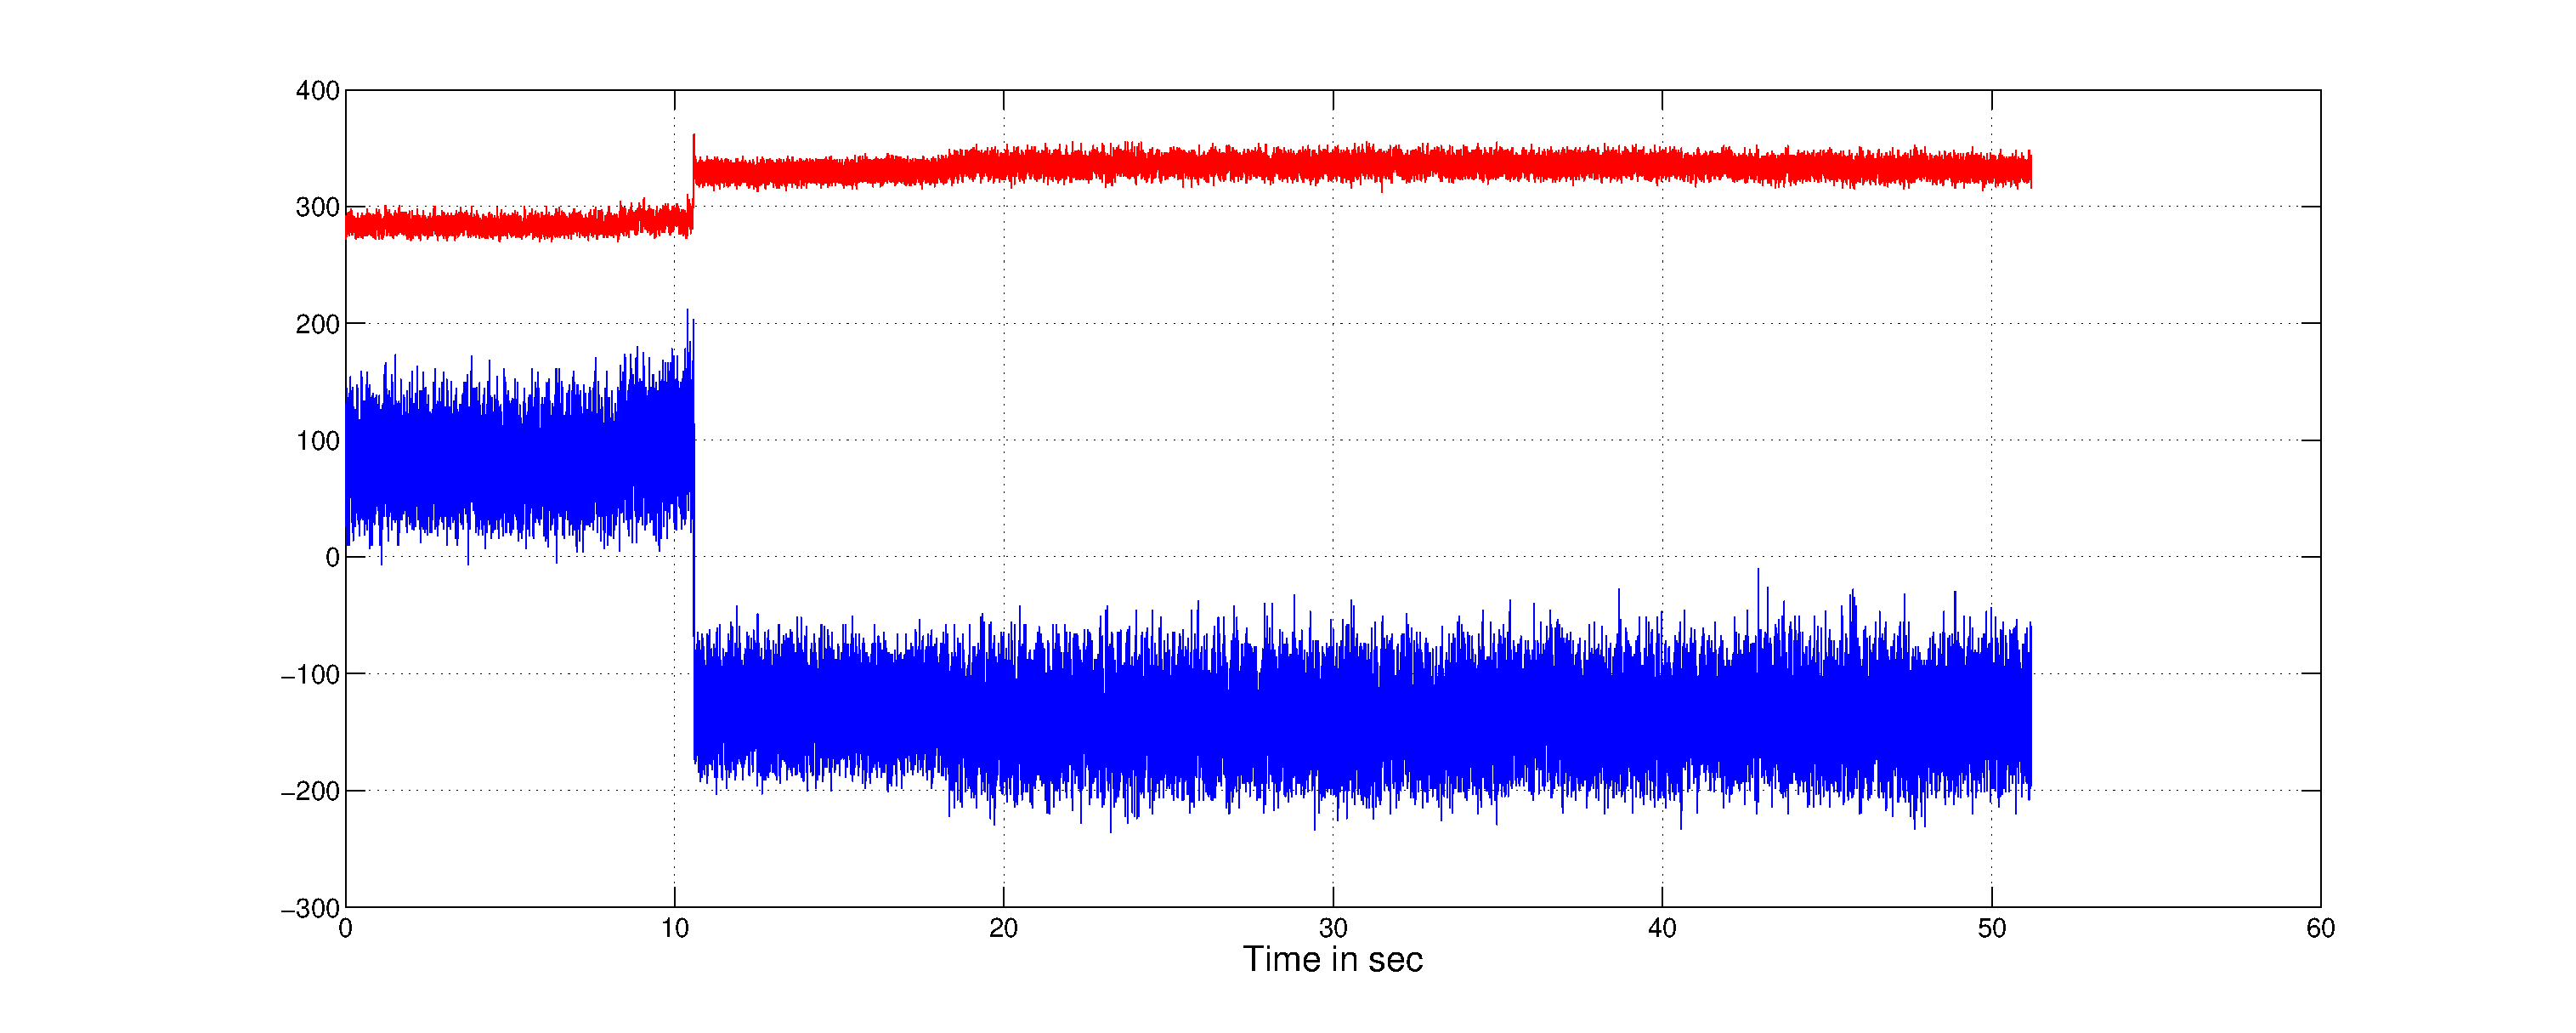
\includegraphics[height=5cm,width=12cm]{I4k_transfer_xb_6.eps}
 %   \caption{Applying step fitting to bead trace}
    \label{fig:graph23}
\end{figure}

\end{frame}

%%-----------------------------------------------------------------------
\begin{frame}{Transition as photodiode O/P} 
Neural Network output
\begin{figure}
    \centering
    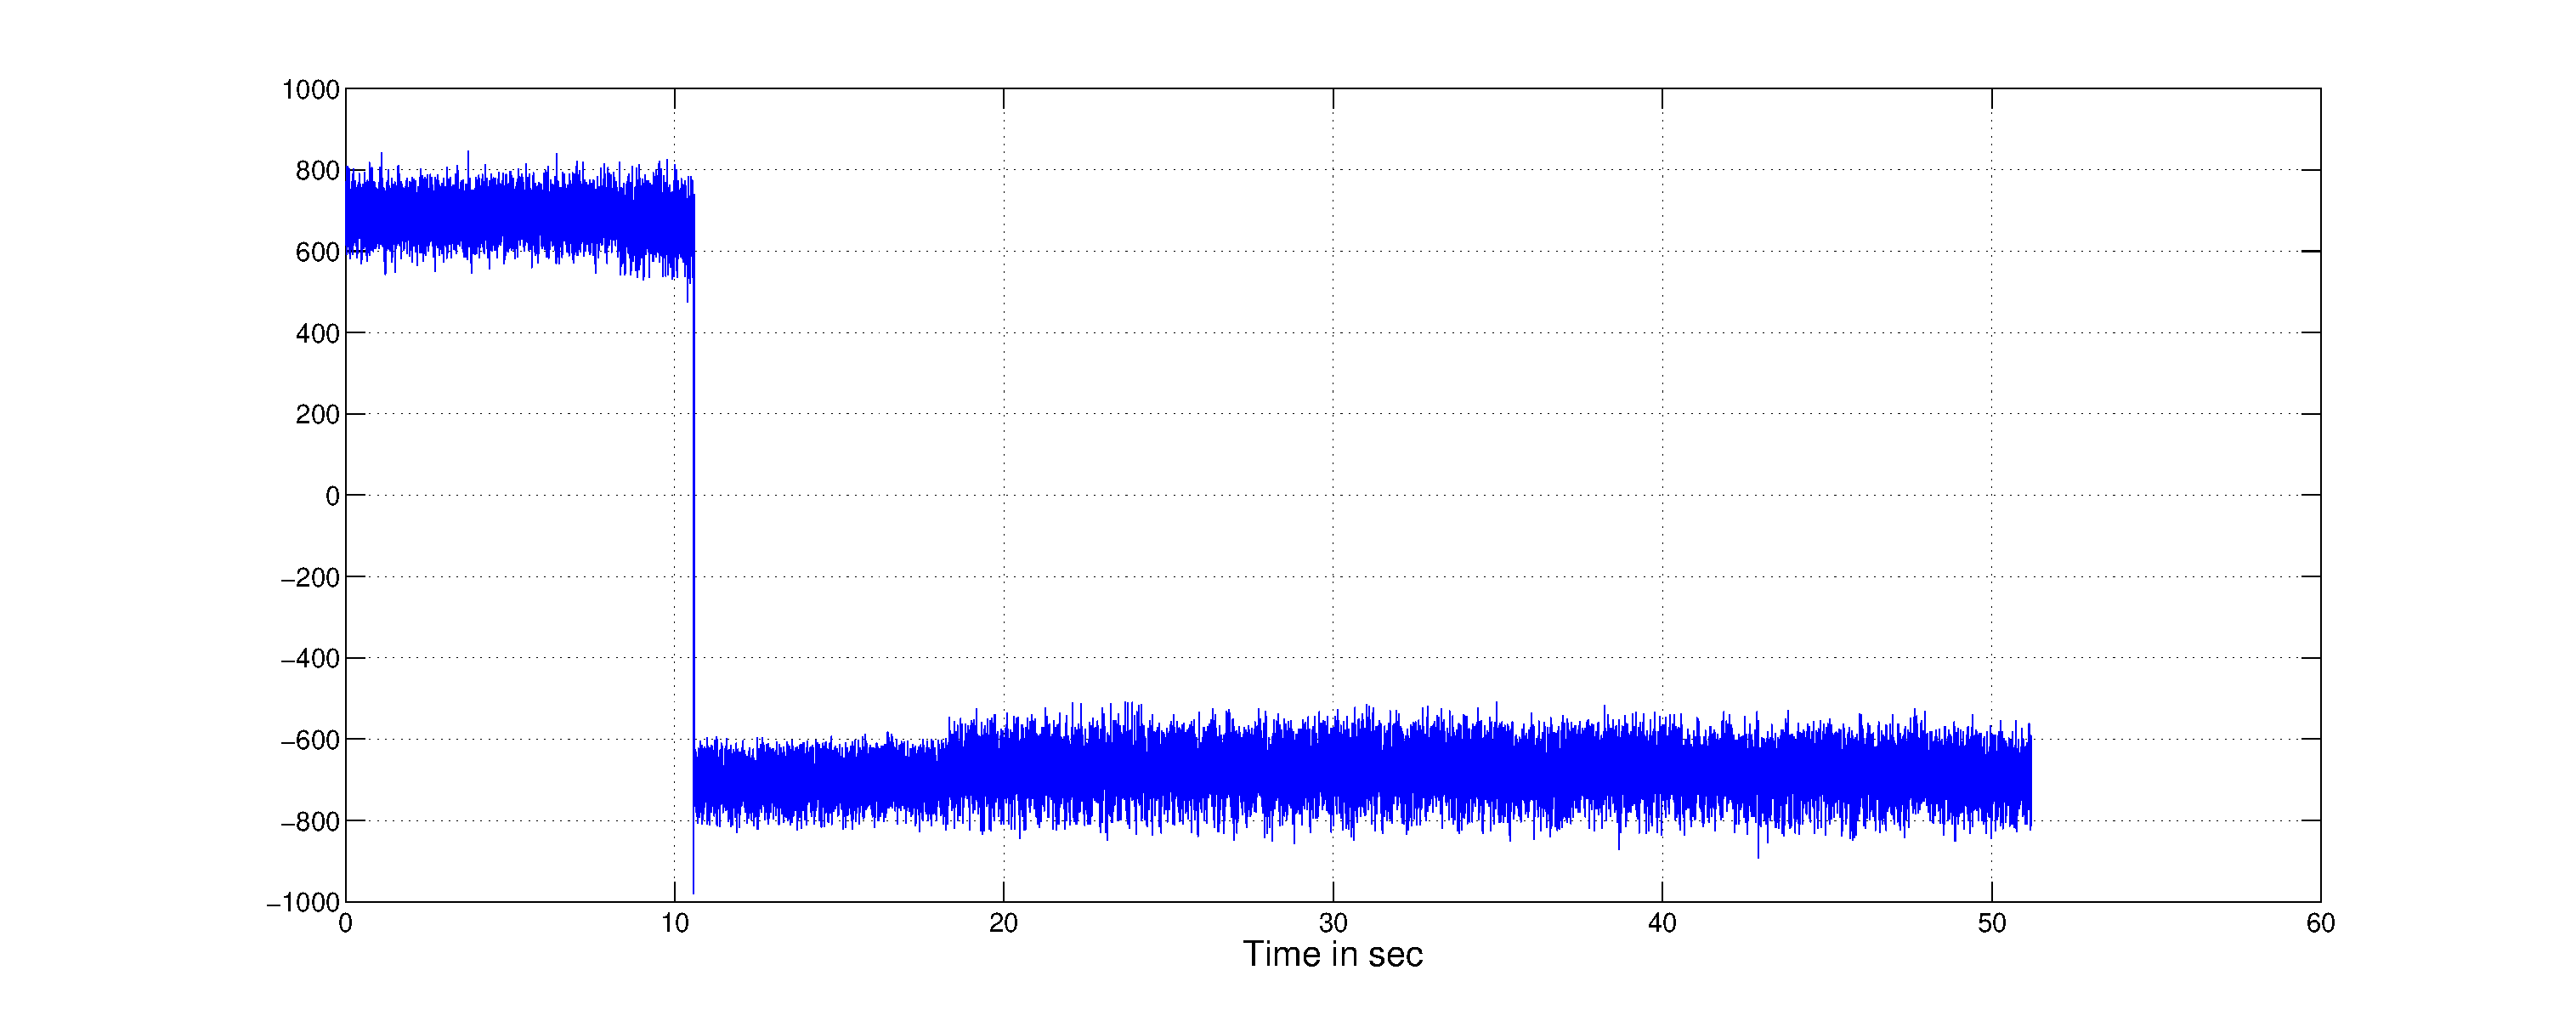
\includegraphics[height=5cm,width=12cm]{I4k_transfer_ActualPos_6.eps}
 %   \caption{Applying step fitting to bead trace}
    \label{fig:graph24}
\end{figure}

\end{frame}

%%-----------------------------------------------------------------------
\begin{frame}{Transition as photodiode O/P} 
Wells during transfer : Blinks L=7 ,R=1 ; L = 2 $K_BT$,R = 3.3 $K_BT$, Height = 12.5 $K_BT$\\
\begin{figure}
    \centering
    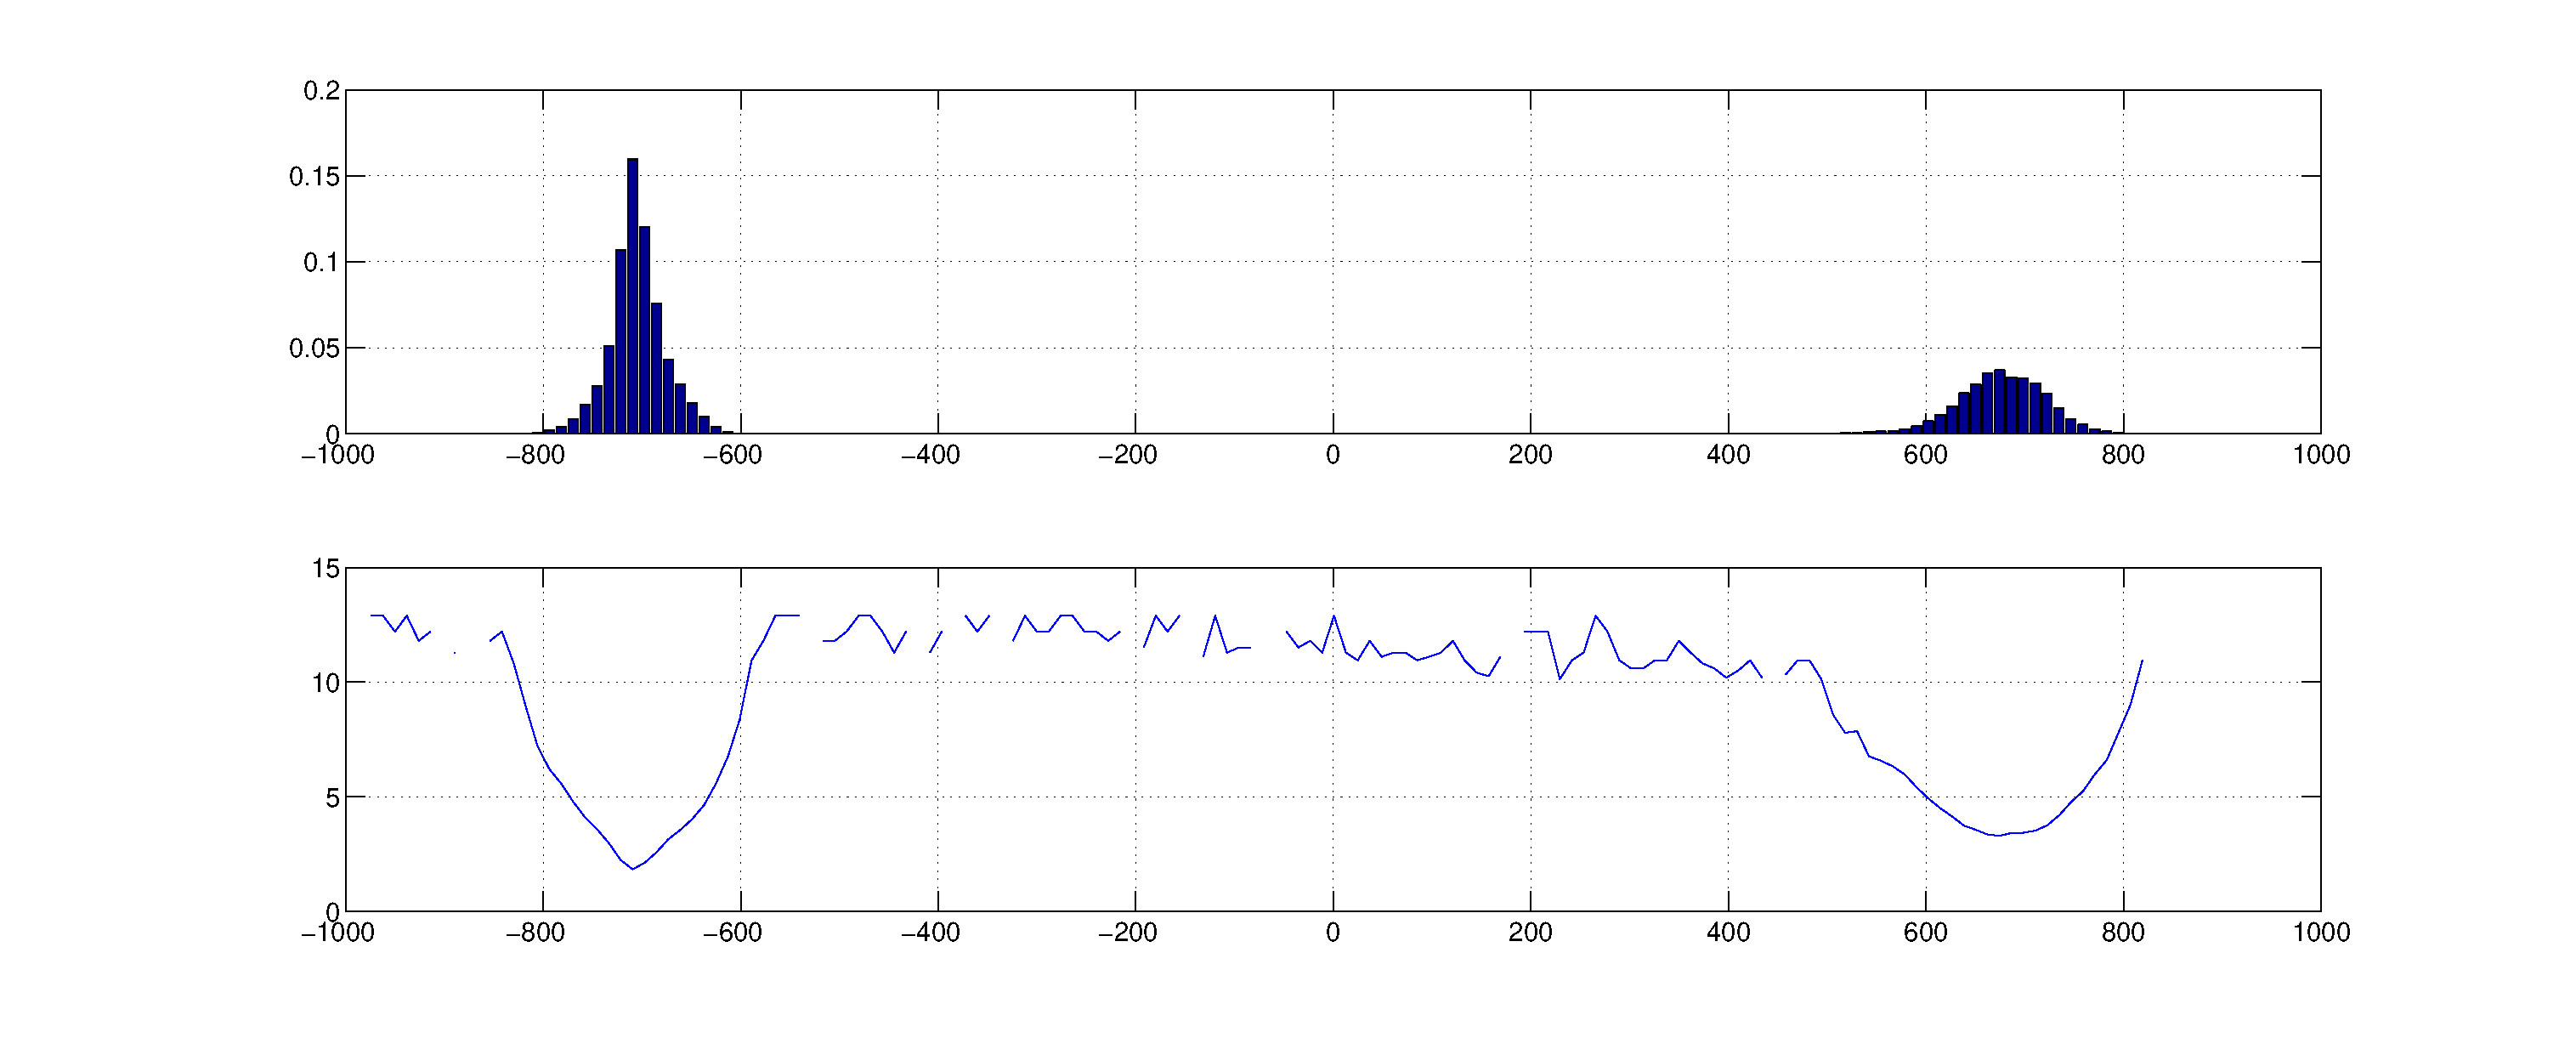
\includegraphics[height=4.5cm,width=12cm]{I4k_transfer_wells_6.eps}
 %   \caption{Applying step fitting to bead trace}
    \label{fig:graph25}
\end{figure}

\end{frame}

%%-----------------------------------------------------------------------
\section{Understanding approach in the Nature paper}
\begin{frame}{What has been done in Nature paper-1} 

\begin{figure}
    \centering
    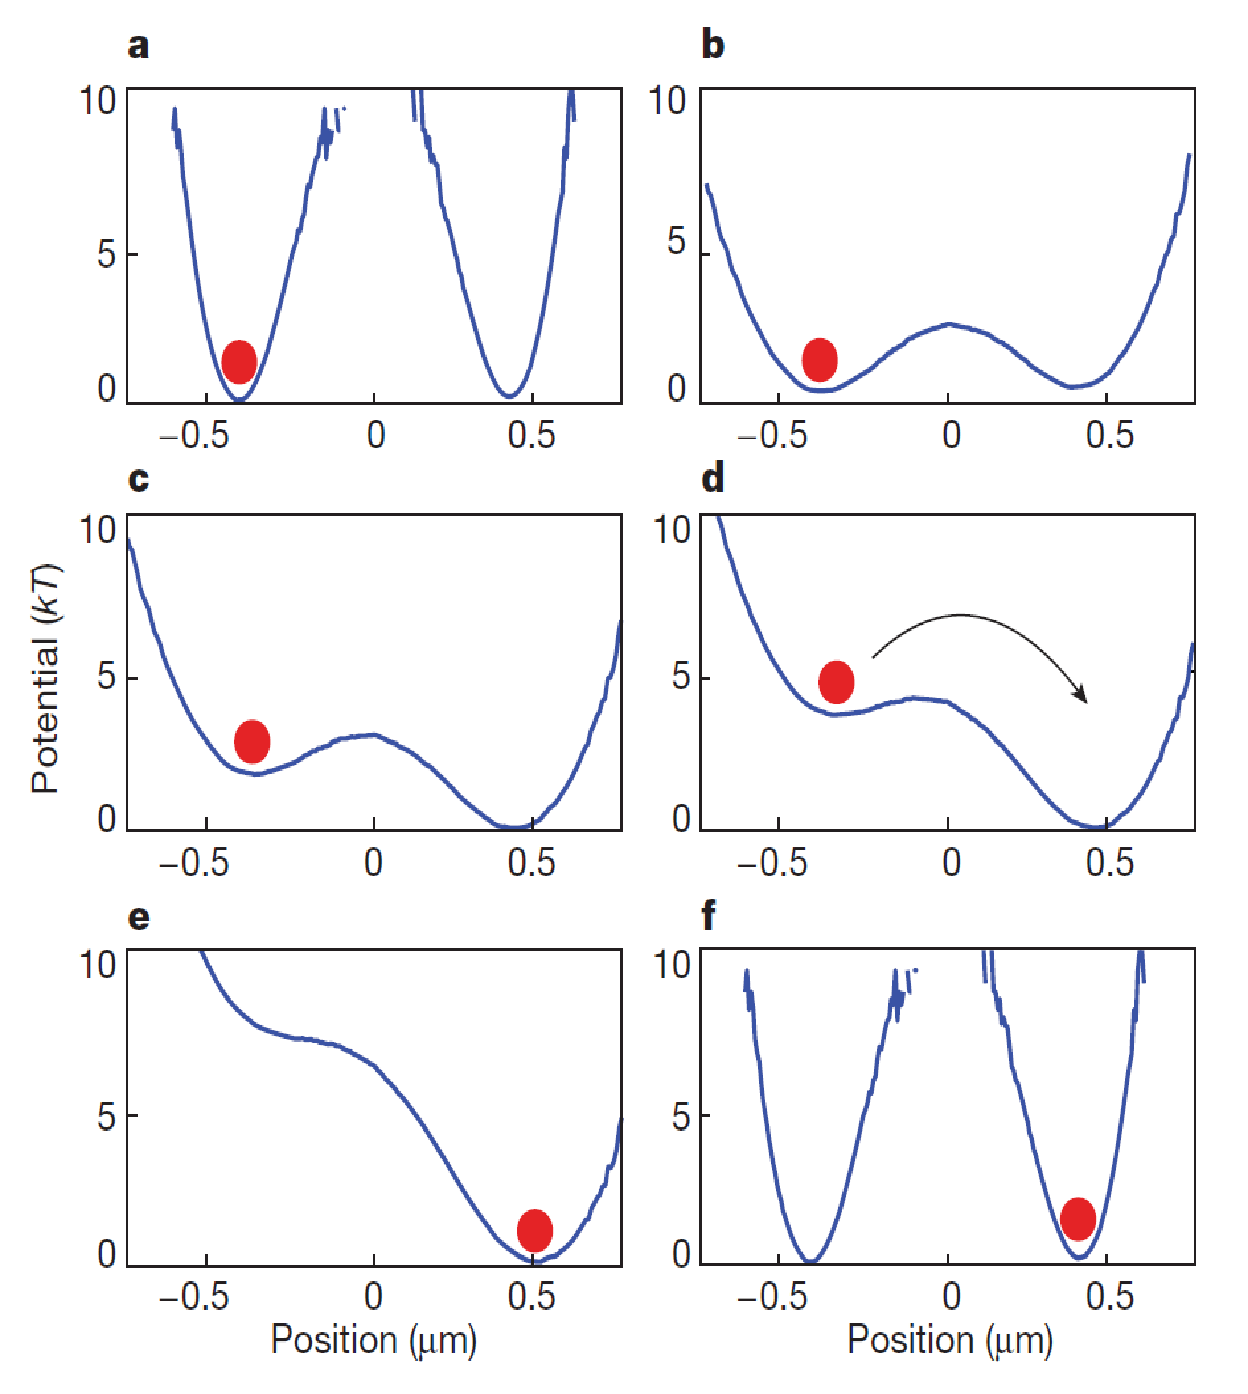
\includegraphics[height=5cm,width=12cm]{nature_landauer_fig1.eps}
 %   \caption{Applying step fitting to bead trace}
    \label{fig:graph26}
\end{figure}

\end{frame}
%%-----------------------------------------------------------------------
\begin{frame}{What has been done in Nature paper-2} 

For fig. a,b and f the plots are found using experimental data as:
\begin{itemize}

\item Well potential calculated using pdf is used via.
\begin{equation*}
U_0(x,I_L) = -K_BT~ln[(P(x,I_L)/N]
\end{equation*}
\item According to paper, the measured $U_0(x,I_L)$ is plotted in fig.a,b,f and can be fitted by $8^{th}$ order polynomial as :
\begin{equation*}
U_0(x,I_L) = \sum_{n=0}^8 u_n(I_L,d_f)x^n
\end{equation*}
where $d_f$ is the distance between the two points over which laser is switched ($1450~nm$ here)

\end{itemize}

\end{frame}
%%-----------------------------------------------------------------------
\begin{frame}{What has been done in Nature paper-3} 

For fig. c,d and e the plots are found using following calculations :
\begin{itemize}

\item Total time of erasure = Time of stage motion with increasing velocity = $\tau$
\item Amplitude of viscous force is increased linearly during time $\tau$ : $F(t)=\pm F_{max}t/\tau$
\item Intermediate plots during transfer is calculated at three different values of time $t$ :
\begin{equation*}
U(x,t) = U_0(x,I_L)- F(t)
\end{equation*}
\item \textit{I suspect, the plot in fig.b is also an $8^{th}$ order fit, since the contours in the plots from b to e are the same}

\end{itemize}

\end{frame}
%%-----------------------------------------------------------------------
\begin{frame}{Our approach-1} 

Replicated fig.a and f with R=3.2 $K_BT$, SD = 48.3 nm, L = 3.4 $K_BT$, SD = 37.1 nm 
\begin{figure}
    \centering
    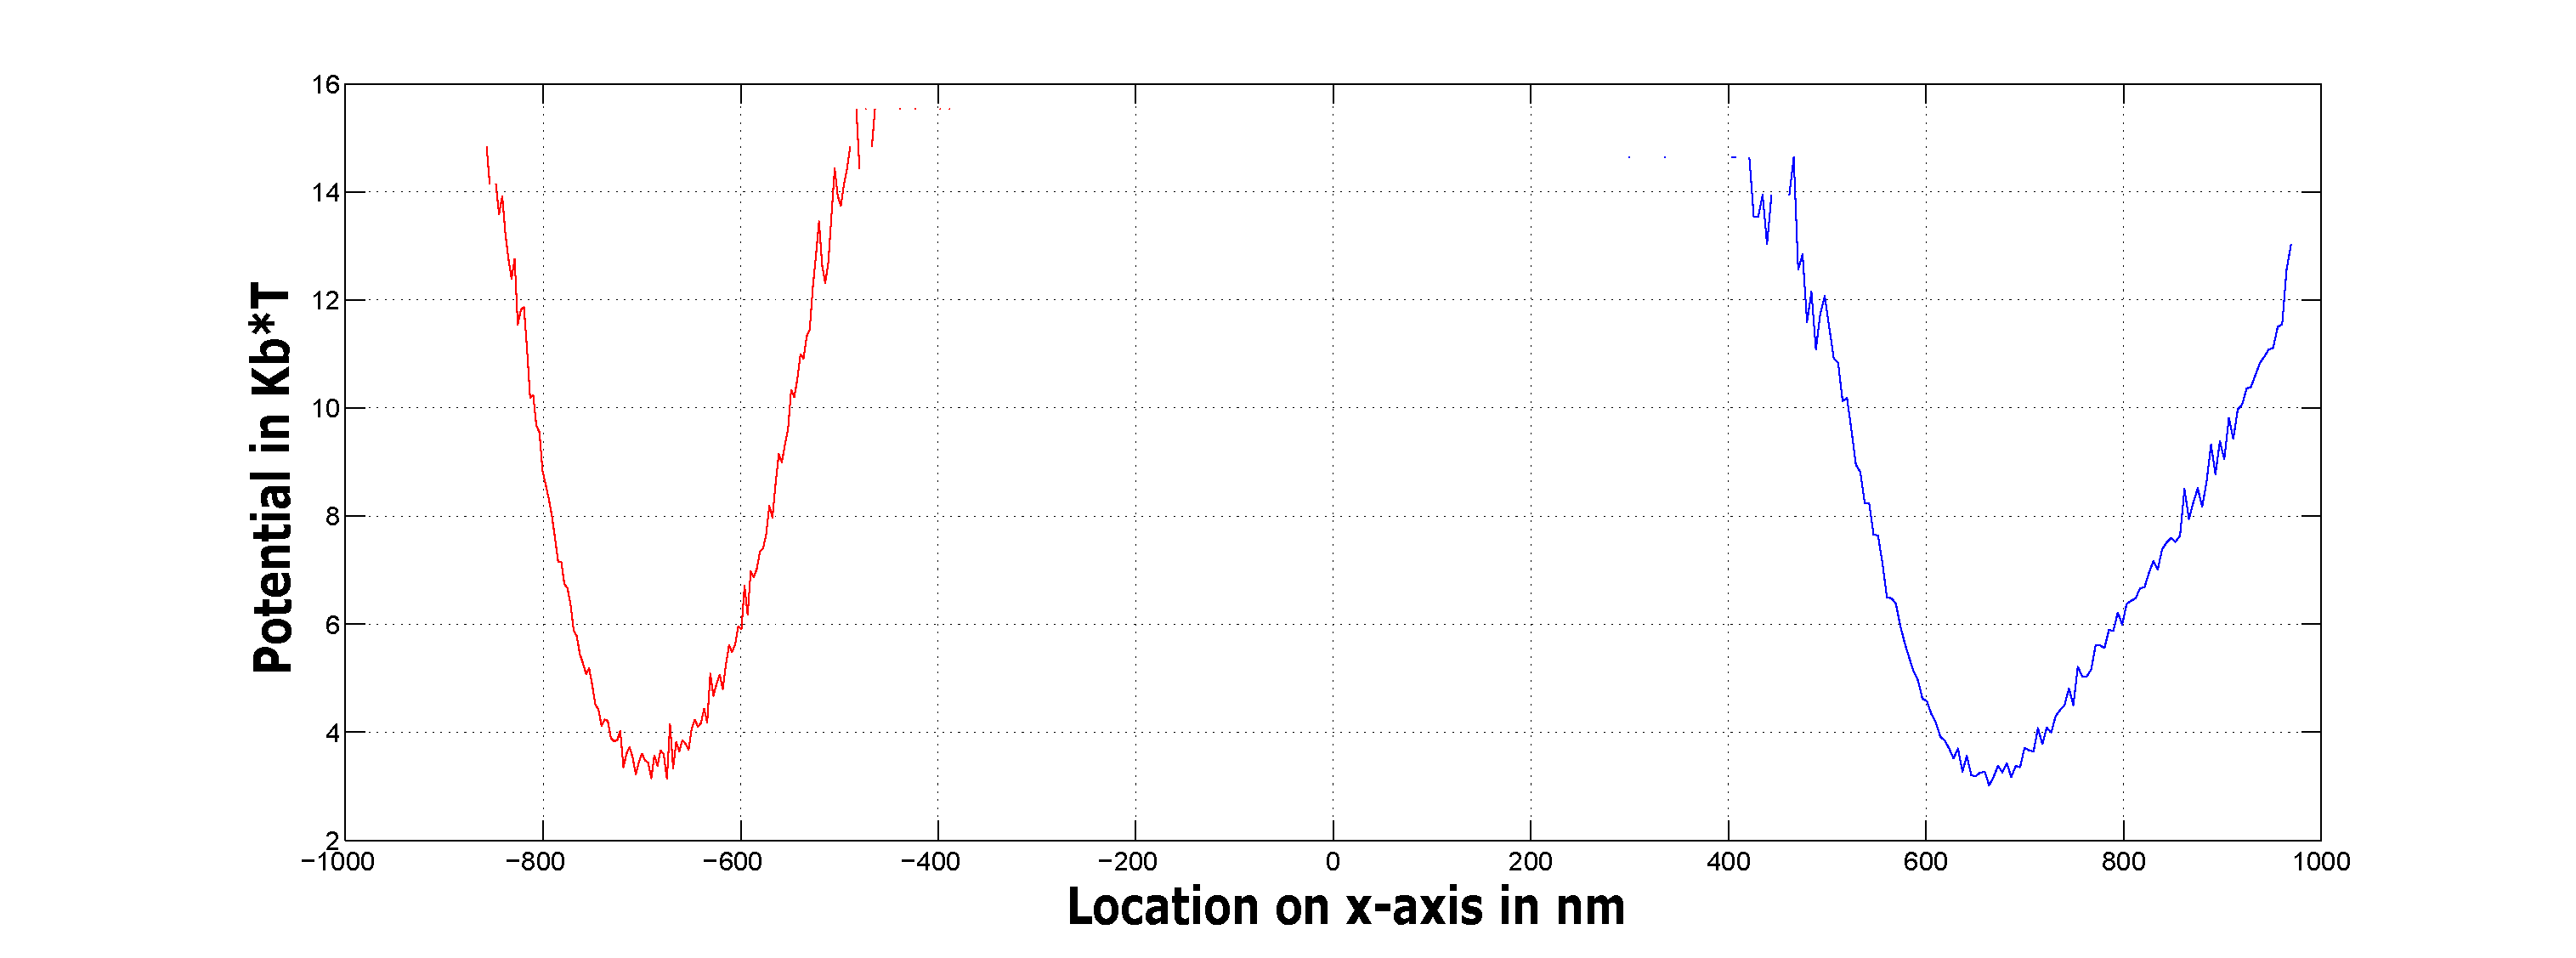
\includegraphics[height=4.5cm,width=12cm]{I4k_both_wells_700_1.eps}
 %   \caption{Applying step fitting to bead trace}

\end{figure}


\end{frame}


%%-----------------------------------------------------------------------
\begin{frame}{Our approach-2} 

Replicated fig.d at exact point of transfer with blinks L=7 ,R=1 ; L = 2 $K_BT$,R = 3.3 $K_BT$, Height = 12.5 $K_BT$
\begin{figure}
    \centering
    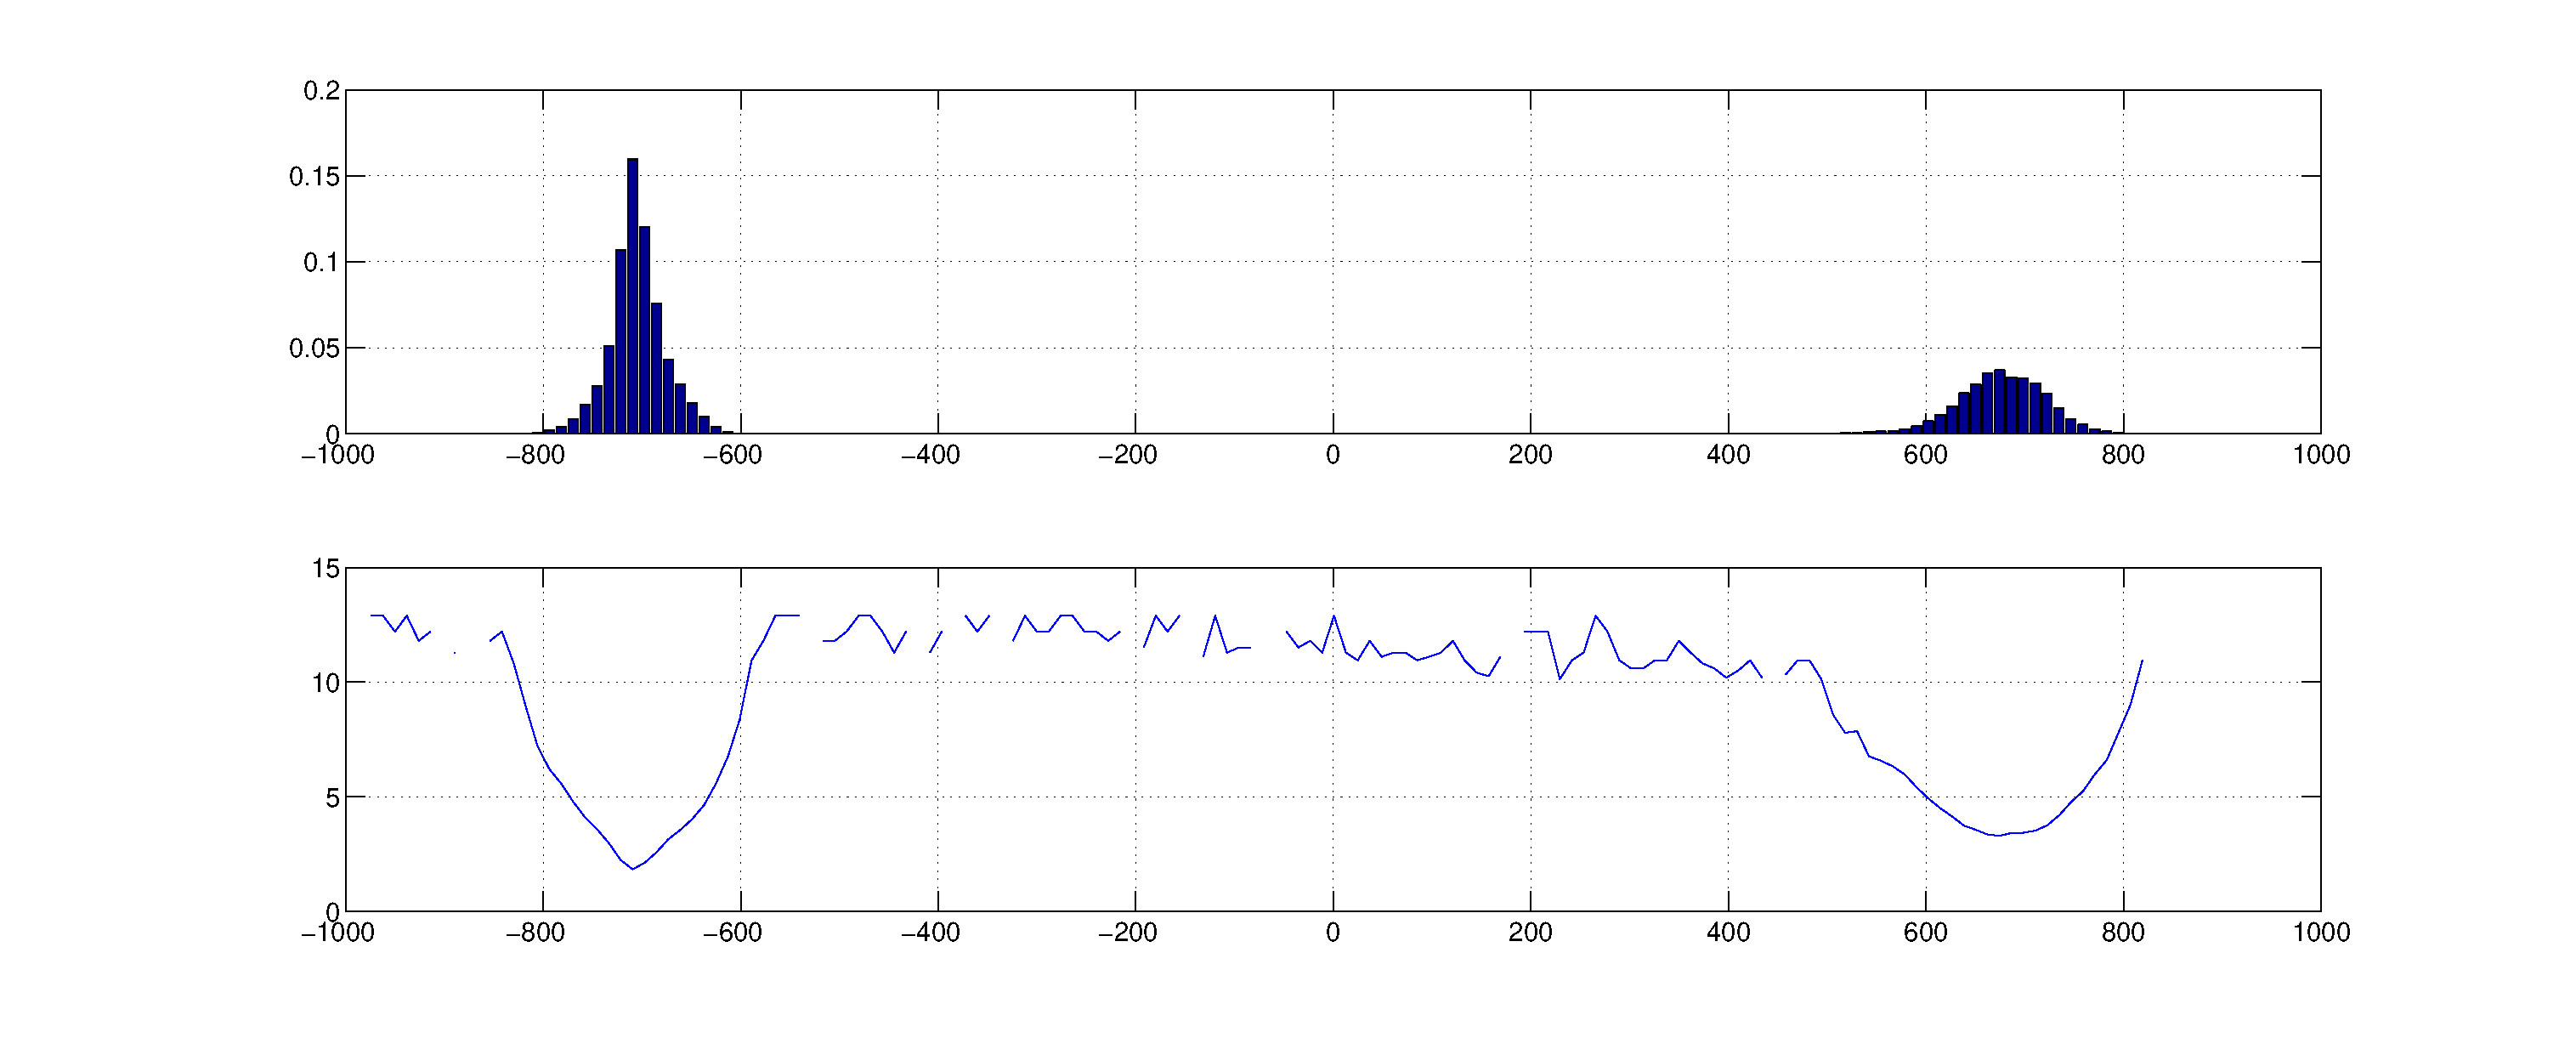
\includegraphics[height=4.5cm,width=12cm]{I4k_transfer_wells_6.eps}
 %   \caption{Applying step fitting to bead trace}
   
\end{figure}


\end{frame}

%%-----------------------------------------------------------------------
\section{Tilting wells - Multiple transfers}
\begin{frame}{Multiple Transfers - Several examples} 

\begin{itemize}

\item Trap bead at +700; potential well formed at +700
\item Total 12 blinks fixed : for equal potential, 6 blinks for each well, each blink for 20 $\mu s$
\item R$\rightarrow$L transition seen from 8,4 onwards i.e. 8,4...9,3...10,2 and 11,1
\item To see the minimum tilt needed for this transition, 8,4 is fixed
\item Modulate the on times as :

\begin{center} 
\begin{tabular}{| l | c | r |} 
\hline Total & Left & Right \\ 
\hline 12 & 6 & 6 \\ 
\hline 12 & 7 & 5 \\ 
\hline 12 & 8 & 4 \\ 
\hline \hline 12 & 6 & 6 \\ 
\hline \end{tabular} 
\end{center}

\end{itemize}

\end{frame}

%%-----------------------------------------------------------------------
\begin{frame}{Averaging 7 instances of R$\rightarrow$L transfer at 8,4 blinks} 

\begin{figure}
    \centering
    \includegraphics[height=5cm,width=11cm]{Mean_of_the_seven_potential_wells_probb1.eps}
 %   \caption{Applying step fitting to bead trace}
    \label{fig:graph27}
\end{figure}

\end{frame}

%%-----------------------------------------------------------------------
\begin{frame}{Inference} 


\end{frame}


%%-----------------------------------------------------------------------
\section{Tilting wells and Work Done}
\begin{frame}{Possible ways to calculate work done} 


\end{frame}
%%-----------------------------------------------------------------------
\begin{frame}{Example 1} 


\end{frame}


%%--------------------------------------------------------------------------------------------------------

%%--------------------------------------------------------------------------------------------------------








\end{document}


